\documentclass[twoside]{ltjsreport}
\usepackage{silence}
\WarningFilter{caption}{Unknown document}
\usepackage[top=20truemm,bottom=20truemm,left=15truemm,right=15truemm,headheight=20pt]{geometry}
\usepackage{fancyhdr,lastpage,abstract,listings,float,wrapfig,tabularx,multirow,multicol}
\usepackage{hyperref,graphics,graphicx,framed,subcaption}
\usepackage[symbol]{footmisc}
\usepackage{amsmath,amssymb}
\usepackage{tikz}
\usetikzlibrary{calc,arrows.meta,fit,positioning,math}
\newcolumntype{A}{>{\centering\bfseries}X}
\newcolumntype{B}{>{\centering\bfseries\arraybackslash}X}
\newcolumntype{C}{>{\centering\arraybackslash}X}
\newcolumntype{R}{>{\raggedright\arraybackslash}X}
\newcolumntype{L}{>{\raggedleft\arraybackslash}X}
\bibliographystyle{junsrt}
\hypersetup{
    colorlinks=true,
    citecolor=black,
    linkcolor=black,
    urlcolor=black
}
\renewcommand{\chaptermark}[1]{\markboth{第\ \thechapter\ 章\,\, #1}{}}
\fancypagestyle{report}{
    \fancyhf{}
    \fancyhead[RE,LO]{\leftmark}
    \fancyfoot[RE,LO]{\thepage\ /\ \pageref{LastPage}}
    \pagenumbering{arabic}
    }
\fancypagestyle{appendixstyle}{
    \fancyhf{}
    \fancyhead[RE,LO]{付録}
    \fancyfoot[RE,LO]{\thepage\ /\ \pageref{LastPage}}
    \renewcommand{\headrulewidth}{0mm}
}
\lstset{
    language = {Matlab},
    %backgroundcolor={\color[gray]{.90}},
    breaklines = true,
    breakindent = 10pt,
    basicstyle = \ttfamily\small,
    commentstyle = {\ttfamily \color[rgb]{0,0.45,0}},
    classoffset = 0,
    keywordstyle = {\bfseries \color{magenta}},
    stringstyle = {\ttfamily \color{blue}},
    frame = left,
    %他オプション:leftline,topline,bottomline,lines,single,shadowbox
    framesep = 5pt,
    numbers = none,
    stepnumber = 1,
    numberstyle = \small,
    tabsize = 4,
    captionpos = t,
    otherkeywords = {xticks, yticks, exportgraphics, imwrite, bitshift, uint8, double}
}
\renewcommand{\figurename}{図}
\renewcommand{\tablename}{表}
\renewcommand{\lstlistingname}{src.}
\renewcommand{\thefootnote}{\fnsymbol{footnote}}
\renewcommand{\contentsname}{目次}
\renewcommand{\listfigurename}{図目次}
\renewcommand{\listtablename}{表目次}
\renewcommand{\lstlistlistingname}{ソースコード}
\renewcommand{\thefigure}{\thechapter-\arabic{figure}}
\renewcommand{\thetable}{\thechapter-\arabic{table}}
\renewcommand{\theequation}{\thechapter.\arabic{equation}}
\renewcommand{\thesubfigure}{(\alph{subfigure})}
\renewcommand{\labelenumi}{\textbf{\theenumi}.\ }
\renewcommand{\eqref}[1]{式(\ref{#1})}
\newcommand{\matlab}{\text{{\large M}ATLAB\raisebox{2mm}{\tiny\textregistered}}}
\newcommand{\mat}[2]{\(#1\)行\(#2\)列}
\newcommand{\figref}[1]{図\ref{#1}}
\newcommand{\tblref}[1]{表\ref{#1}}
\newcommand{\srcref}[1]{src.\ref{#1}}
\newcommand{\scall}[1]{課題\ (#1)\ のスクリプトは,}
\newcommand{\sref}[1]{\(\underset{\blacktriangleright\textrm{p.\pageref{#1}}}{\textrm{\srcref{#1}}}\)}
\captionsetup[subfigure]{labelformat=simple}
\makeatletter
\@addtoreset{figure}{chapter}
\@addtoreset{table}{chapter}
\@addtoreset{lstlisting}{chapter}
\@addtoreset{footnote}{page}
\renewcommand{\chapter}{%
    \if@openright\cleardoublepage\else\clearpage\fi
    \global\@topnum\z@
    \secdef\@chapter\@schapter}
\makeatother
\AtBeginDocument{
    \renewcommand{\thelstlisting}{\thechapter-\arabic{lstlisting}}
}
\title{{\normalsize 情報学群実験第3C/3i 実験レポート 第2回}\\画像情報と視覚情報の処理に関する実験}
\author{1250373\hspace{1\zw}溝口 洸熙\thanks{高知工科大学 情報学群 情報セキュリティシステム研究室}\\Group 10}
\date{May 28th, 2023}
\begin{document}
% paragraph command
\newcommand{\purpose}{\subsection{実験の目的}}
\newcommand{\method}{\subsection{実験の方法と考え方}}
\newcommand{\result}{\subsection{実験の結果}}
\newcommand{\consideration}{\subsection{考察}}
\newcommand{\conclusion}{\subsection{結論}}
% 課題1
\newcommand{\kadaiaa}{カラーチャネル操作}
\newcommand{\kadaiab}{画像の量しかビット数変換}
\newcommand{\kadaiac}{階調反転}
\newcommand{\kadaiad}{閾値処理}
\newcommand{\kadaiae}{ヒストグラム}
% 課題2
\newcommand{\kadaiba}{テスト画像作成}
\newcommand{\kadaibb}{平滑化フィルタ・メディアンフィルタ}
\newcommand{\kadaibc}{微分フィルタ}
\newcommand{\kadaibd}{ラプラシアンフィルタ}
\newcommand{\kadaibe}{色空間変換}
\maketitle
\renewcommand{\abstractname}{概要}
\begin{abstract}
    本実験では,画像情報処理,視覚情報処理を扱う.画像情報処理では,カラーチャネル操作や閾値処理,量子化数変換などの基礎的な画像処理を行い,それらの技術を用いて画像フィルタや背景差分画像の作成や肌色領域の抽出,2次元フーリエ変換を行う.2次元フーリエ変換のパワースペクトルと原画像の関係や,2次元フーリエ変換後の出力と,画像座標との関係が明らかになった.また,背景差分画像と色空間変換後の肌色領域抽出で,対象物の抽出における特徴も明らかとなった.
    視覚情報処理では,方位残効を扱う.\matlab 上で方位残効刺激を作成する.この実験より,縞模様方位の大きさと,方位残効の度合いの関係を,ヒトの視覚情報処理を考慮した上で明らかになった.
\end{abstract}
\pagenumbering{roman}\thispagestyle{plain}
\tableofcontents
\listoffigures
\lstlistoflistings
\newpage
\pagestyle{report}
\setcounter{page}{1}
\chapter{画像情報処理}
\section{\purpose}
\matlab を用いて,画像に対して,カラーチャネルの操作,量子化数変換,階調反転,閾値処理,画素値に対するヒストグラムを作成など,基本的な画像処理を行う.\par
また,HSV色空間上での肌色抽出する.HSV色空間の特徴として,人間が色を知覚する方法と類似しており,視覚障害者向けのアクセシビリティ向上に役立つことが挙げられる\cite[p.97\ -\ p.98]{画像処理}.\par
人間が色を知覚する方法と類似していることを踏まえて,HSV色空間を用いることで,画像の特徴を抽出しやすくなる.今回の実験では,自分の手の写真をRGB色空間からHSV色空間へ変換し,肌色領域を抽出する.抽出した肌色領域を白色,そのほかの部分を黒色にして出力する.出力した画像と,RGB色空間における肌色領域を抽出した場合の精度について考察する.\par
さらに,ノイズ画像に対して,ノイズ除去する.周囲画素値の平均値を中央の画素値にする平滑化フィルタと,周囲画素値の中央値を中央の画素値にするメディアンフィルタを,ノイズの雑音除去具合で比較する.\par
画像のエッジを検出するために,微分フィルタを適用する.
画像を2次元フーリエ変換し,パワースペクトルを出力する.出力したパワースペクトルに対して,周波数フィルタを適用し,結果を考察する.
\paragraph{\kadaiaa}RGB色空間の画像を,緑チャネルだけを抜き出してグレイスケール画像を作成する.赤チャネル,青チャネルについても同様にグレイスケール画像を生成する.さらに,RGB画像の赤チャネルと青チャネルを入れ替えたカラー画像を作成する.
\paragraph{\kadaiab}グレイスケール画像を生成する.緑チャネルは色の濃淡を多く含む.RGB色空間から色の濃淡を抽出したい場合は,緑(G)の成分を多く抽出するとよい.具体的な割合を,\eqref{equ:grayscale}に示す.ここではNTSC輝度信号を取り出す方法で行う.生成したグレイスケール画像に対して,画像の量子化数を変更することによる,画像の変化を確認する.量子化数は8Bit,4Bit,2Bit,1Bitの4種をテストする.量子化数1Bitの画像を2値画像という.
\begin{align}
    \textrm{Gray scale image} & = \textrm{Red}\times 30\% +\textrm{Green}\times 59\% +\textrm{Blue}\times 11\%\label{equ:grayscale}
\end{align}
\paragraph{\kadaiac}各量子化数の画像に対して,その画像を階調反転させる.階調反転とは,白黒を反転させることである.量子化数による階調変換後の画像を比較する.
\paragraph{\kadaiad}閾値処理とは,とある値(閾値)以上の場合を白,閾値以下を黒とし,2値画像を作成することである.
\paragraph{\kadaiae}量子化数8Bitのグレイスケール画像のヒストグラムを作成する.画素値\(n(n=0,1,\dots ,255)\)の画素が何画素含まれているかのヒストグラムを作成する.
\paragraph{\kadaiaf}自分が写っている写真と,背景だけが写っている写真の差分画像をとる.これを背景差分と呼ぶ.背景差分の後,閾値処理を行う.物体領域を正しく検出するために考慮する点を考察する.
\paragraph{画像フィルタ} 画像に対して,フィルタを適用するとはどのようなことか?我々は,携帯電話の写真アプリケーションを用いて,写真を「加工」する.
我々は「加工」という行為を「フィルタをかける」と呼ぶが,この「フィルタ」という言葉と,画像処理におけるフィルタは意味が異なる.
画像処理におけるフィルタは,画像ないに含まれる雑音を除去したり,特徴を抽出したりすることで欠陥検出をより円滑に行うための基本処理を指す\cite{画像フィルタ}.
\newcommand{\originimg}{\texttt{original\_img}}
\newcommand{\wgnimg}{\texttt{wgn\_img}}
\newcommand{\inimg}{\texttt{in\_img}}
テスト画像として,以下の画像を用意する.グレイスケール元画像を\originimg とする.
\begin{enumerate}
    \item \textbf{白色ガウス雑音}\\
          白色ガウス雑音は,白色性を持つガウス雑音である.今回は,平均\(0\),標準偏差\(10\)としてガウス分布の乱数を発生させる.
          このテスト画像を\wgnimg とする.
    \item \textbf{インパルス雑音}\\
          インパルス雑音とは.超短時間におこる高周波の雑音のことを指す.今回は,画像のランダムな画素を,白または黒で塗り替える.それぞれ全体画素の1\(\%\) の割合で作成する.
          このテスト画像を\inimg とする.
\end{enumerate}
画像フィルタはいくつかの種類があり,画像雑音の除去やエッジの強調に用いられる.
\begin{enumerate}
    \item \textbf{平滑化フィルタ}
          \begin{itemize}
              \item 画像の各画素\(p\)に対して,\(n\)近傍と中央の画素値の平均や重み付け平均をとり,\(p\)の画素値とするフィルタ.
              \item 今回の実験では,各画素\(p\)に対して,\(3\times 3\),つまり8近傍と\(p\)の画素値の平均をとり,中央の画素値として定義する.2つのテスト画像にフィルタを適用し,雑音とフィルタの関係を考察する.
          \end{itemize}
    \item \textbf{メディアンフィルタ}
          \begin{itemize}
              \item 画像の各画素\(p\)に対して,\(n\)近傍と中央の画素値を昇順に整列し,その中央値を\(p\)の画素値とする.
              \item 今回の実験では,各画素\(p\)に対して,\(3\times 3\),つまり8近傍と\(p\)の画素値を昇順に整列する.その中央値を\(p\)の画素値として定義する.2つのテスト画像にフィルタを適用し,雑音とフィルタの関係を考察する.
          \end{itemize}
    \item \textbf{微分フィルタ}
          \begin{itemize}
              \item 微分フィルタは,境界線の強調や局所的な特徴の抽出するフィルタである.しかし,1次微分フィルタ,2次微分フィルタを用いると,画像の雑音も強調される.ここでPrewittフィルタとSobelフィルタを用いると,雑音がある画像でもうまく境界線を抽出できる\cite[p.87]{画像処理}.
                    \begin{itemize}
                        \item \textbf{Prewitt フィルタ}:隣り合う2画素の画素値を持ちいて3画素ずつをセットにして濃度の変化点を抽出するアルゴリズム\cite[p.87]{画像処理}.
                        \item \textbf{Sobel フィルタ}:画像の各ピクセルの周囲の画素との差を計算して,その差の大きさを使って,エッジを検出するアルゴリズム.
                    \end{itemize}
              \item 今回の実験では,\originimg に対して,Sobelフィルタを用いて縦微分,横微分,縦微分と横微分の加算合成した画像を作成する.フィルタを適用した画像の特徴と,それぞれの違いを考察する.
          \end{itemize}
    \item \textbf{Laplacianフィルタ}
          \begin{itemize}
              \item Laplacianフィルタは,微分フィルタ同様,境界線を見つけるために使われる方法である.
              \item 今回の実験では,\originimg に対して,Laplacianフィルタを適用し,閾値処理する.フィルタを適用し閾値処理した画像と特徴と違いを考察する.
          \end{itemize}
\end{enumerate}
\begin{figure}[h]
    \centering
    \begin{minipage}[b]{.24\textwidth}
        \centering
        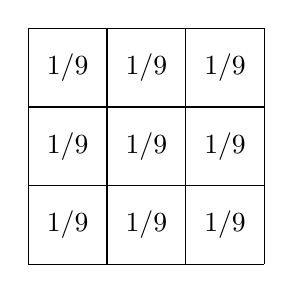
\begin{tikzpicture}
            \draw (0,0) grid (3,3);
            \foreach \u \v in {0.5/0.5,1.5/0.5,2.5/0.5,0.5/1.5,1.5/1.5,2.5/1.5,0.5/2.5,1.5/2.5,2.5/2.5}
            \node at (\u,\v) {\(1/9\)};
        \end{tikzpicture}
        \subcaption{平滑化フィルタ}
        \label{fig:平滑化フィルタ}
    \end{minipage}
    \begin{minipage}[b]{.24\textwidth}
        \centering
        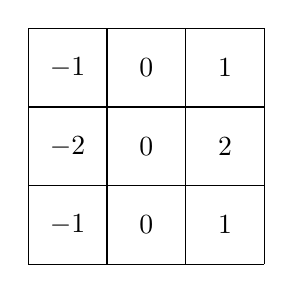
\begin{tikzpicture}
            \draw (0,0) grid (3,3);
            \foreach \u \v \w in {0.5/0.5/{\(-1\)},1.5/0.5/{\(0\)},2.5/0.5/{\(1\)},0.5/1.5/{\(-2\)},1.5/1.5/{\(0\)},2.5/1.5/{\(2\)},0.5/2.5/{\(-1\)},1.5/2.5/{\(0\)},2.5/2.5/{\(1\)}}
            \node at (\u,\v) {\w};
        \end{tikzpicture}
        \subcaption{Sobelフィルタ:横方向}
        \label{fig:Prewittフィルタ_横方向}
    \end{minipage}
    \begin{minipage}[b]{.24\textwidth}
        \centering
        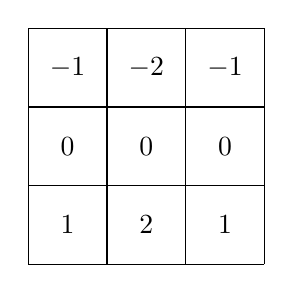
\begin{tikzpicture}
            \draw (0,0) grid (3,3);
            \foreach \u \v \w in {0.5/0.5/{\(1\)},1.5/0.5/{\(2\)},2.5/0.5/{\(1\)},0.5/1.5/{\(0\)},1.5/1.5/{\(0\)},2.5/1.5/{\(0\)},0.5/2.5/{\(-1\)},1.5/2.5/{\(-2\)},2.5/2.5/{\(-1\)}}
            \node at (\u,\v) {\w};
        \end{tikzpicture}
        \subcaption{Sobelフィルタ:縦方向}
        \label{fig:Prewittフィルタ_縦方向}
    \end{minipage}
    \begin{minipage}[b]{.24\textwidth}
        \centering
        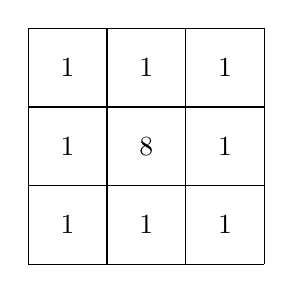
\begin{tikzpicture}
            \draw (0,0) grid (3,3);
            \foreach \u \v in {0.5/0.5,1.5/0.5,2.5/0.5,0.5/1.5,2.5/1.5,0.5/2.5,1.5/2.5,2.5/2.5}
            \node at (\u,\v) {\(1\)};
            \node at (1.5,1.5) {\(8\)};
        \end{tikzpicture}
        \subcaption{Laplacianフィルタ}
        \label{fig:Laplacianフィルタ}
    \end{minipage}
    \caption{\(3\times 3\)画像フィルタ}
\end{figure}
\paragraph{色空間変換}この実験では,RGB色空間から,HSV色空間へ変換する.RGB色空間は,赤(Red),緑(Green),青(Blue)の3チャネルで構成する.HSVは色相(Hue),彩度(Saturation),明度(Value)の3チャネルで構成する.
色相は,カラー ホイール上の色の位置に対応する,\(0\)から\(100\)の値,色相の量または中間からの逸脱.特定の色の赤,緑,青成分の中での最大値.いずれも\texttt{double}型で保存される\cite{rgb2hsv}.
\paragraph{2次元フーリエ変換}
フーリエ変換は,任意の連続信号に対して各空間周波数成分が,どの程度含まれているかを示す変換である.音声などの1次元信号に対しては,離散1次元フーリエ変換を適用した.画像は2次元信号なので,2次元離散フーリエ変換し,空間周波数成分を取り出す.
出力されるスペクトルは,縦軸に\(y\)方向のスペクトル,横軸には\(x\)方向のスペクトル,輝度には成分の大きさが表現されている.
今回の実験では,\matlab を用いて,画像に対して2次元フーリエ変換し,パワースペクトルを作成する.
実際の画像とパワースペクトルを比較し,画像上の座標との関係や,パワースペクトルが何を示しているか明らかにする.
さらに,画像に対して高域通過フィルタを適用し,パワースペクトルが表す意味を考察する.
\section{\method}
\subsection{装置と用語解説}
この実験にはMathWorks\raisebox{2mm}{\tiny\textregistered}社の\matlab を用いて,\tblref{tbl:実験環境}の環境下で実験する.
\begin{table}[H]
    \caption{実験環境}
    \label{tbl:実験環境}
    \begin{tabularx}{\columnwidth}{cR}
        \hline
        \multirow{2}{*}{実験機}   & MacBook Air 2022 (Apple社)   \\
                               & 型番:\texttt{MLY13J/A}        \\
        \hline
        \multirow{2}{*}{プロセッサ} & Apple Silicon M2            \\
                               & 8コアCPU,8コアGPU               \\
        \hline
        メモリ                    & 8GB                         \\
        \hline
        ブラウザ                   & Safari\ バージョン16.5           \\
        \hline
        ImageJ                 & 1.53k\ Java 13.0.6 (64-bit) \\
        \hline
    \end{tabularx}
\end{table}
\paragraph{HTML}
Hyper Text Markup Languageの略で,Webページを作成するためのマークアップ言語.Webページ上のテキストデータに「タグ」を与えて,文字の大きさ,色やフォントを変更する.
\paragraph{CSS}
Cascading Style Sheetsの略で,Webページのスタイルを指定するための言語である.CSSの適用により,ホームページの文字や背景などがタグを利用して統一される.
\paragraph{JavaScript}
ブラウザ上で動作するアプリケーションを記述するための言語である.現在のWebアプリケーション上でデファクトスタンダード言語である\cite[p.68]{CGとゲームの技術}.
\subsection{JavaScriptの初歩}
\begin{itemize}
    \item \textbf{\texttt{A.indexOf("Strings")}}\\
          JavaScriptには,\texttt{A.indexOf("Strings")}で,\texttt{Strings}が\texttt{A}に含まれているかどうか出力する関数がある.
    \item \textbf{ユーザエージェント(UA)}\\
          ユーザエージェント(UA)とは,利用者のブラウザとOSを指す.
          この実験で利用するUAは,macOSのSafariである.
          SafariにはUAを変更する機能がある.Chrome,Firefox,MicrosoftEdge,Safari 16.4は,SafariのUA切り替え機能を用いて実験する.
\end{itemize}
\kadai{ブラウザ判定}\par
\texttt{Navigator object}オブジェクトの\texttt{userAgent}プロパティを用いて,利用ブラウザの判定を行う.
\texttt{A}に\texttt{Strings}が含まれていない場合,戻り値は\texttt{-1}である.この実験では,ブラウザがFirefoxである場合は\ \texttt{this browser is Firefox}\ ,そうでない場合は\ \texttt{this browser is not Firefox}\ と表示するWebページを作成する.\\
\kadai{ブラウザによるCSSの切り替え}\par
ブラウザ判定を用いて,ブラウザによってCSSを変更するJavaScriptを記述する.CSSを設定する\texttt{link}タグに\texttt{id}を指定し,\texttt{document.getElementById}関数で\texttt{link}タグをインスタンス化する.
ブラウザ判定結果により,このインスタンスを利用してCSSを変更する.この実験では,CSSで背景色のみを変更する.UAと指定背景色は\tblref{tbl:UAと指定背景色}に示す.
\begin{table}[H]
    \centering
    \caption{UAと指定背景色}
    \label{tbl:UAと指定背景色}
    \begin{tabularx}{\columnwidth}{RRR}
        \multicolumn{1}{c}{UA} & \multicolumn{1}{c}{背景色}    & \multicolumn{1}{c}{CSS名} \\
        \hline
        Firefox                & \rulebox{{orange}}{orange} & \texttt{firefox.css}     \\
        Chrome                 & \rulebox{{blue}}{blue}     & \texttt{chrome.css}      \\
        Other                  & \rulebox{{gray}}{gray}     & \texttt{default.css}     \\
        \hline
    \end{tabularx}
\end{table}
ここで,MicrosoftEdgeは,UAに\texttt{"Chrome"}文字列と\texttt{"Edge"}文字列を持つ.正確にUA\texttt{Chrome}を判別するには,条件式に,「\texttt{"Chrome"}を含み\texttt{"Edge"}を除く」処理を記述する必要がある.\\
\kadai{時刻によるCSSの切り替え}\par
JavaScriptで現在時刻を取得するには,\texttt{Date}をインスタンス化する必要がある.\texttt{Date}内の\texttt{getSeconds}関数を呼び出すことで,現在時刻の「秒」を得られる.
この実験では,現在時刻\footnote{正確には,HTMLを読み込んだ時刻.}の秒数を\(n\)とすると,以下の条件でCSSを変更する.
\begin{equation*}
    \textrm{適用するCSS}=
    \begin{cases}
        \texttt{firefox.css} & (0\leq n<20)  \\
        \texttt{chrome.css}  & (20\leq n<40) \\
        \texttt{default.css} & (40\leq n<60)
    \end{cases}
\end{equation*}
\kadai{マウスイベントの取得}\par
この実験では,「現在時刻の取得」と書かれた文字上をクリックすると,クリックした時刻をリストとして後ろに追加するプログラムを記述する.文字列「現在時刻の取得」をひとつのオブジェクトとして定義するため,\texttt{<span></span>}タグを用いる.
また,リストアイテムとして表示するために,現在時刻を\texttt{<ul></ul>}タグ内の要素\texttt{<li></li>}タグへ格納する.\par
\begin{enumerate}
    \item 「現在時刻の取得」文字列を\texttt{<p></p>}タグの属性\texttt{onmousedown}で,現在時刻をリストアイテムとして追加する関数\texttt{input\_item()}を呼び出す.この関数を呼び出すと,変数\texttt{time}に,時刻\texttt{Hour:Minutes:Second}が格納される.
    \item \texttt{<ul></ul>}に対して,\texttt{document.getElementById}関数を用いてインスタンス名\texttt{list}でインスタンス化する.
    \item \texttt{document.createElement("li")}関数で,\texttt{<li></li>}タグを生成し,変数\texttt{listItem}に格納する.
    \item \texttt{listItem}の要素を\texttt{listItem.textContent}で指定し,\texttt{time}を代入する.
    \item \texttt{list.appendChild(listItem)}で\texttt{listitem}を子要素として組み込む.
\end{enumerate}
\subsection{色覚}
色覚は,以下のように説明されている.
\begin{quotation}
    ``光の刺激により色を見分ける感覚.''\hfill\cite{2020新明解国語辞典}
\end{quotation}
すべての色は,光の三原色と呼ばれる「赤」「緑」「青」から構成される.
色を感じとる視細胞も,赤緑青それぞれに敏感な細胞が3種類存在する.
色覚異常はこの3種類の視細胞のうちどれか足りなかったり,十分に機能しないために起こる.
\begin{figure}[H]
    \centering
    \caption{各視細胞の光に対する感度}
    \label{fig:各視細胞の光に対する感度}
    \begin{tikzpicture}
        \draw[-latex](0,0)--(5.7,0)node[midway,below=.4cm]{\small 光の波長(nm)};
        \draw[-latex](0,0)--(0,3)node[midway,left]{\small \rotatebox{90}{光に対する感度}};
        \foreach \u \v in {0.3/400,1.3/450,2.3/500,3.3/550,4.3/600,5.3/650}
        \draw(\u,-0.1)node[below]{\scriptsize \v}--(\u,0.1);
        \draw[very thick,blue,dotted](0.3,0.5)..controls (1.0,2.8)..(2.3,1.2);
        \draw[very thick,green!50!gray,dashed](1.0,0.5)..controls (2.5,2.8)..(4.9,0.5);
        \draw[thick, red](2.0,0.8)..controls (3.8,2.8)..(5.4,0.8);
    \end{tikzpicture}
    \begin{tikzpicture}
        \draw[very thick,blue,dotted](0,0)--(2,0)node[right,color=black]{青に敏感な視細胞(S錐体)};
        \draw[very thick,green!50!gray,dashed](0,-.5)--(2,-.5)node[right,color=black]{緑に敏感な視細胞(M錐体)};
        \draw[thick,red](0,-1)--(2,-1)node[right,color=black]{赤に敏感な視細胞(L錐体)};
    \end{tikzpicture}
\end{figure}
\begin{table}[H]
    \centering
    \caption{色覚}
    \label{tbl:色覚}
    \begin{tabularx}{\columnwidth}{lR}
        \multicolumn{1}{c}{色覚} & \multicolumn{1}{c}{状態}          \\
        \hline
        C型色覚                   & 3錐体が正常.一般色覚.                    \\
        P型色覚                   & {\small L錐体に異常がある.赤色と灰色の識別が困難.} \\
        D型色覚                   & {\small M錐体に異常がある.緑色と灰色の識別が困難.} \\
        T型色覚                   & S錐体に異常がある.青色と黄色が混同.             \\
        \hline
    \end{tabularx}
\end{table}
講義一覧,折れ線グラフ,円グラフを4つの色覚に対応できるように設計する.\\
\kadai{講義一覧の作成}\par
HTMLの\texttt{table}タグを用いて,講義一覧を作成する.各講義の「専門基礎科目」,「専門発展科目」,「専門領域科目」の背景色と,履修登録必須科目の文字色を,CSSで設定する.
デフォルトのセル背景配色を\tblref{tbl:デフォルト配色}に示す.
また,履修登録必須科目は,\texttt{<p1></p1>}タグ内の\texttt{color}属性で指定し,色を\rulebox{[HTML]{ff0000}}{\#ff0000}とする.
\begin{table}[H]
    \centering
    \caption{デフォルト配色}
    \label{tbl:デフォルト配色}
    \begin{tabularx}{\columnwidth}{RRR}
        \multicolumn{1}{c}{分類} & \multicolumn{1}{c}{セル背景色}          & \multicolumn{1}{c}{\texttt{class}名} \\
        \hline
        専門基礎科目                 & \rulebox{[HTML]{55bb55}}{\#55bb55} & \texttt{kiso}                       \\
        専門発展科目                 & \rulebox{[HTML]{ff9900}}{\#ff9900} & \texttt{hatten}                     \\
        専門領域科目                 & \rulebox{[HTML]{66aaaa}}{\#66aaaa} & \texttt{ryouiki}                    \\
        \hline
    \end{tabularx}
\end{table}

\section{\result}
\begin{figure}[H]
    \centering
    \begin{minipage}[b]{.19\textwidth}
        \centering
        
\includegraphics[keepaspectratio,width=\textwidth]{../../kut.jpg}
        \subcaption{元画像}
        \label{fig:元画像}
    \end{minipage}
    \begin{minipage}[b]{.19\textwidth}
        \centering
        
\includegraphics[keepaspectratio,width=\textwidth]{../../Figures/05_11_r.png}
        \subcaption{赤チャネル}
    \end{minipage}
    \begin{minipage}[b]{.19\textwidth}
        \centering
        
\includegraphics[keepaspectratio,width=\textwidth]{../../Figures/05_12_g.png}
        \subcaption{緑チャネル}
    \end{minipage}
    \begin{minipage}[b]{.19\textwidth}
        \centering
        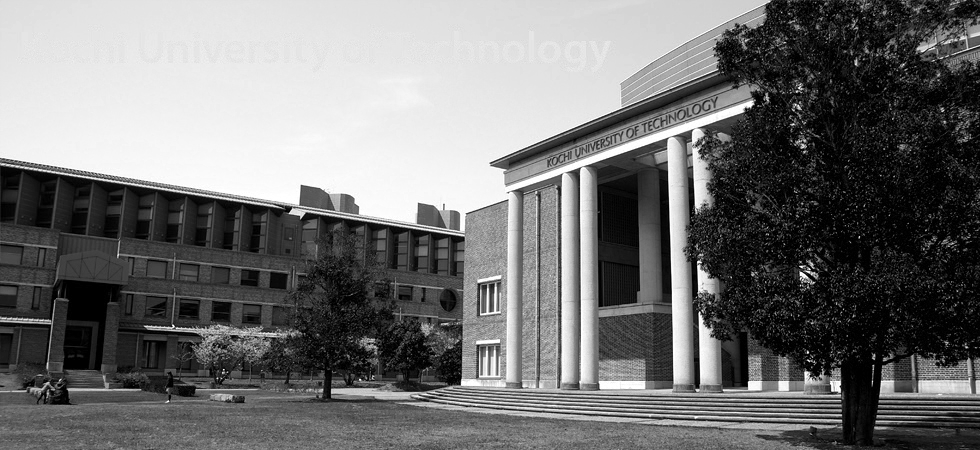
\includegraphics[keepaspectratio,width=\textwidth]{../../Figures/05_13_b.png}
        \subcaption{青チャネル}
    \end{minipage}
    \begin{minipage}[b]{.19\textwidth}
        \centering
        
\includegraphics[keepaspectratio,width=\textwidth]{../../Figures/05_14_change.png}
        \subcaption{赤青チャネル入れ替え}
    \end{minipage}
    \caption{\kadaiaa\ 実験結果}
\end{figure}
\begin{figure}[H]
    \centering
    \begin{minipage}[b]{.23\textwidth}
        \centering
        
\includegraphics[keepaspectratio,width=\textwidth]{../../Figures/05_21_gimg.png}
        \subcaption{量子化数\ 8Bit\footnotemark[1]}
    \end{minipage}
    \begin{minipage}[b]{.23\textwidth}
        \centering
        
\includegraphics[keepaspectratio,width=\textwidth]{../../Figures/05_22_4bit.png}
        \subcaption{量子化数\ 4Bit}
    \end{minipage}
    \begin{minipage}[b]{.23\textwidth}
        \centering
        
\includegraphics[keepaspectratio,width=\textwidth]{../../Figures/05_23_2bit.png}
        \subcaption{量子化数\ 2Bit}
    \end{minipage}
    \begin{minipage}[b]{.23\textwidth}
        \centering
        
\includegraphics[keepaspectratio,width=\textwidth]{../../Figures/05_24_1bit.png}
        \subcaption{量子化数\ 1Bit}
    \end{minipage}
    \caption{\kadaiab\ 実験結果}
\end{figure}
\begin{figure}[H]
    \centering
    \begin{minipage}[b]{.23\textwidth}
        \centering
        
\includegraphics[keepaspectratio,width=\textwidth]{../../Figures/05_31_8.png}
        \subcaption{量子化数\ 8Bit}
    \end{minipage}
    \begin{minipage}[b]{.23\textwidth}
        \centering
        
\includegraphics[keepaspectratio,width=\textwidth]{../../Figures/05_32_4.png}
        \subcaption{量子化数\ 4Bit}
    \end{minipage}
    \begin{minipage}[b]{.23\textwidth}
        \centering
        
\includegraphics[keepaspectratio,width=\textwidth]{../../Figures/05_33_2.png}
        \subcaption{量子化数\ 2Bit}
    \end{minipage}
    \begin{minipage}[b]{.23\textwidth}
        \centering
        
\includegraphics[keepaspectratio,width=\textwidth]{../../Figures/05_34_1.png}
        \subcaption{量子化数\ 1Bit}
    \end{minipage}
    \caption{\kadaiac\ 実験結果}
\end{figure}
\begin{figure}[H]
    \centering
    \begin{minipage}[b]{.7\textwidth}
        \centering
        \begin{minipage}[b]{.3\textwidth}
            \centering
            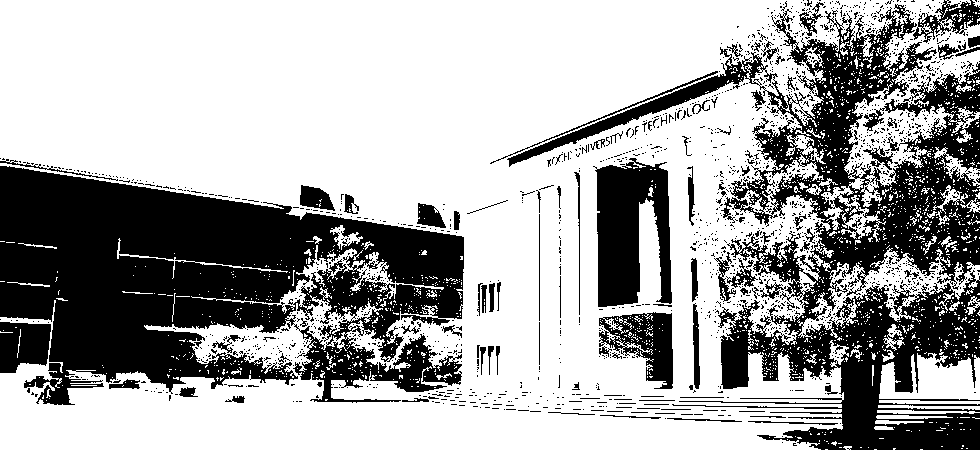
\includegraphics[keepaspectratio,width=\textwidth]{../../Figures/05_41.png}
            \subcaption{閾値\ \(64\)}
        \end{minipage}
        \begin{minipage}[b]{.3\textwidth}
            \centering
            
\includegraphics[keepaspectratio,width=\textwidth]{../../Figures/05_42.png}
            \subcaption{閾値\ \(128\)}
        \end{minipage}
        \begin{minipage}[b]{.3\textwidth}
            \centering
            
\includegraphics[keepaspectratio,width=\textwidth]{../../Figures/05_43.png}
            \subcaption{閾値\ \(192\)}
        \end{minipage}
        \caption{\kadaiad\ 実験結果}
    \end{minipage}
    \begin{minipage}[b]{.25\textwidth}
        \centering
        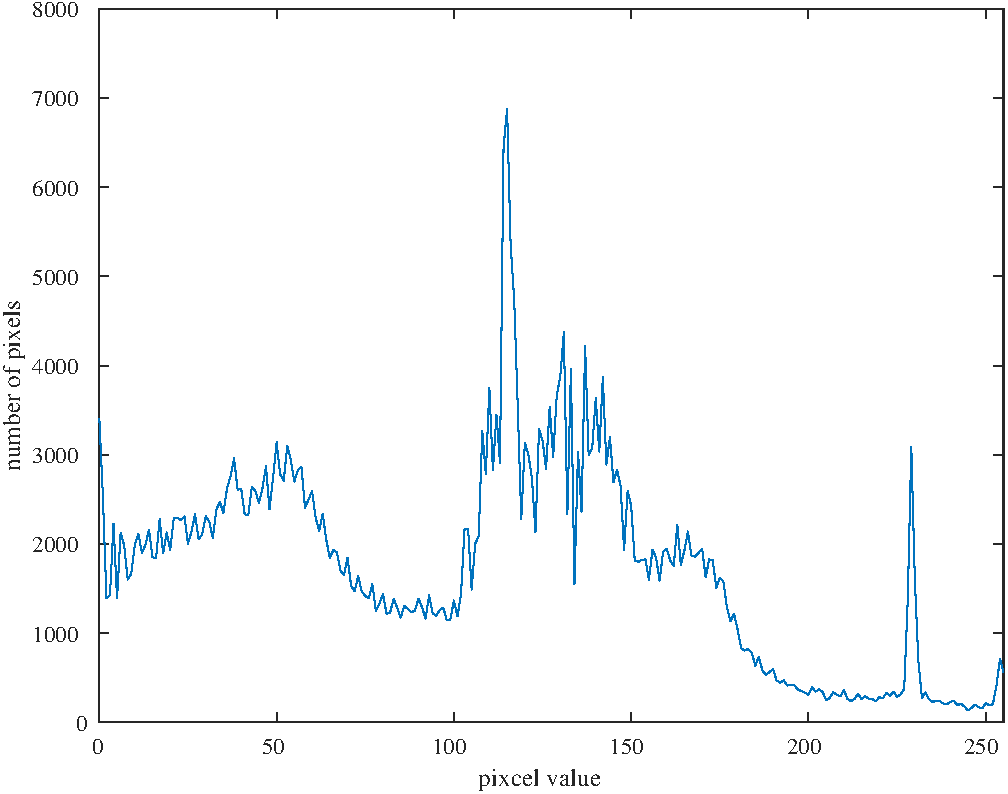
\includegraphics[keepaspectratio,width=\textwidth]{../../Figures/05_50_graph.pdf}
        \caption{\kadaiae\ 実験結果}
    \end{minipage}
\end{figure}
\begin{figure}[H]
    \centering
    \begin{minipage}[b]{.49\textwidth}
        \centering
        \begin{minipage}[b]{.3\textwidth}
            \centering
            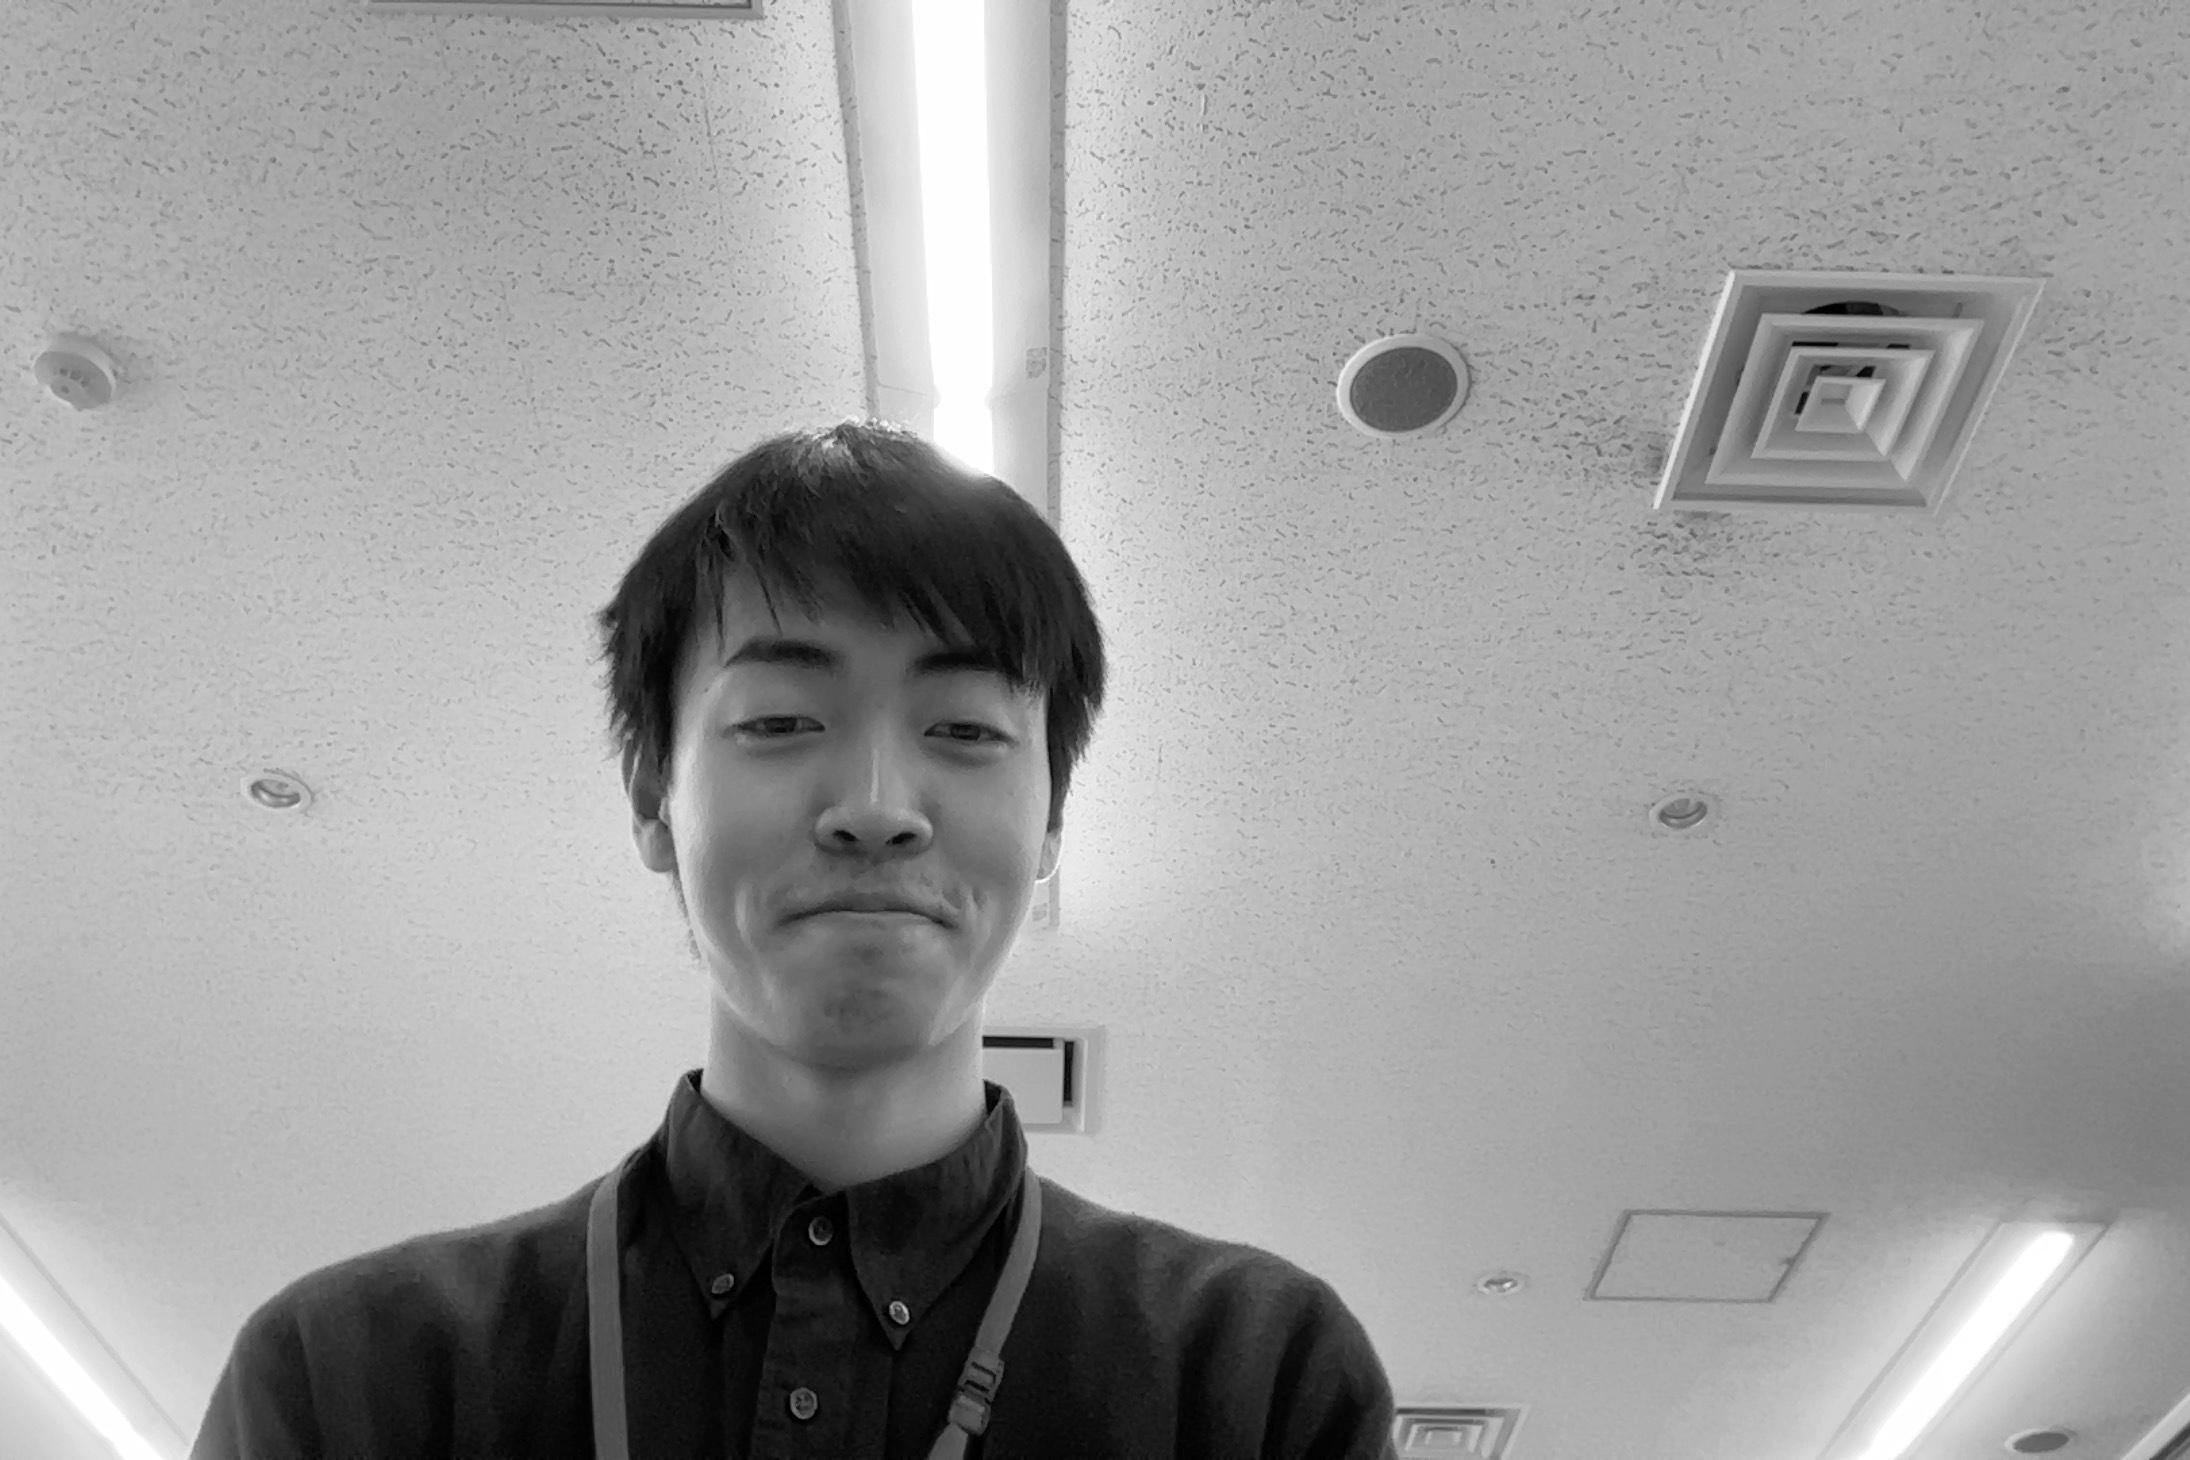
\includegraphics[keepaspectratio,width=\textwidth]{../../05_UnderstandingImages/fig1_g.jpg}
            \subcaption{被写体と背景}
        \end{minipage}
        \begin{minipage}[b]{.3\textwidth}
            \centering
            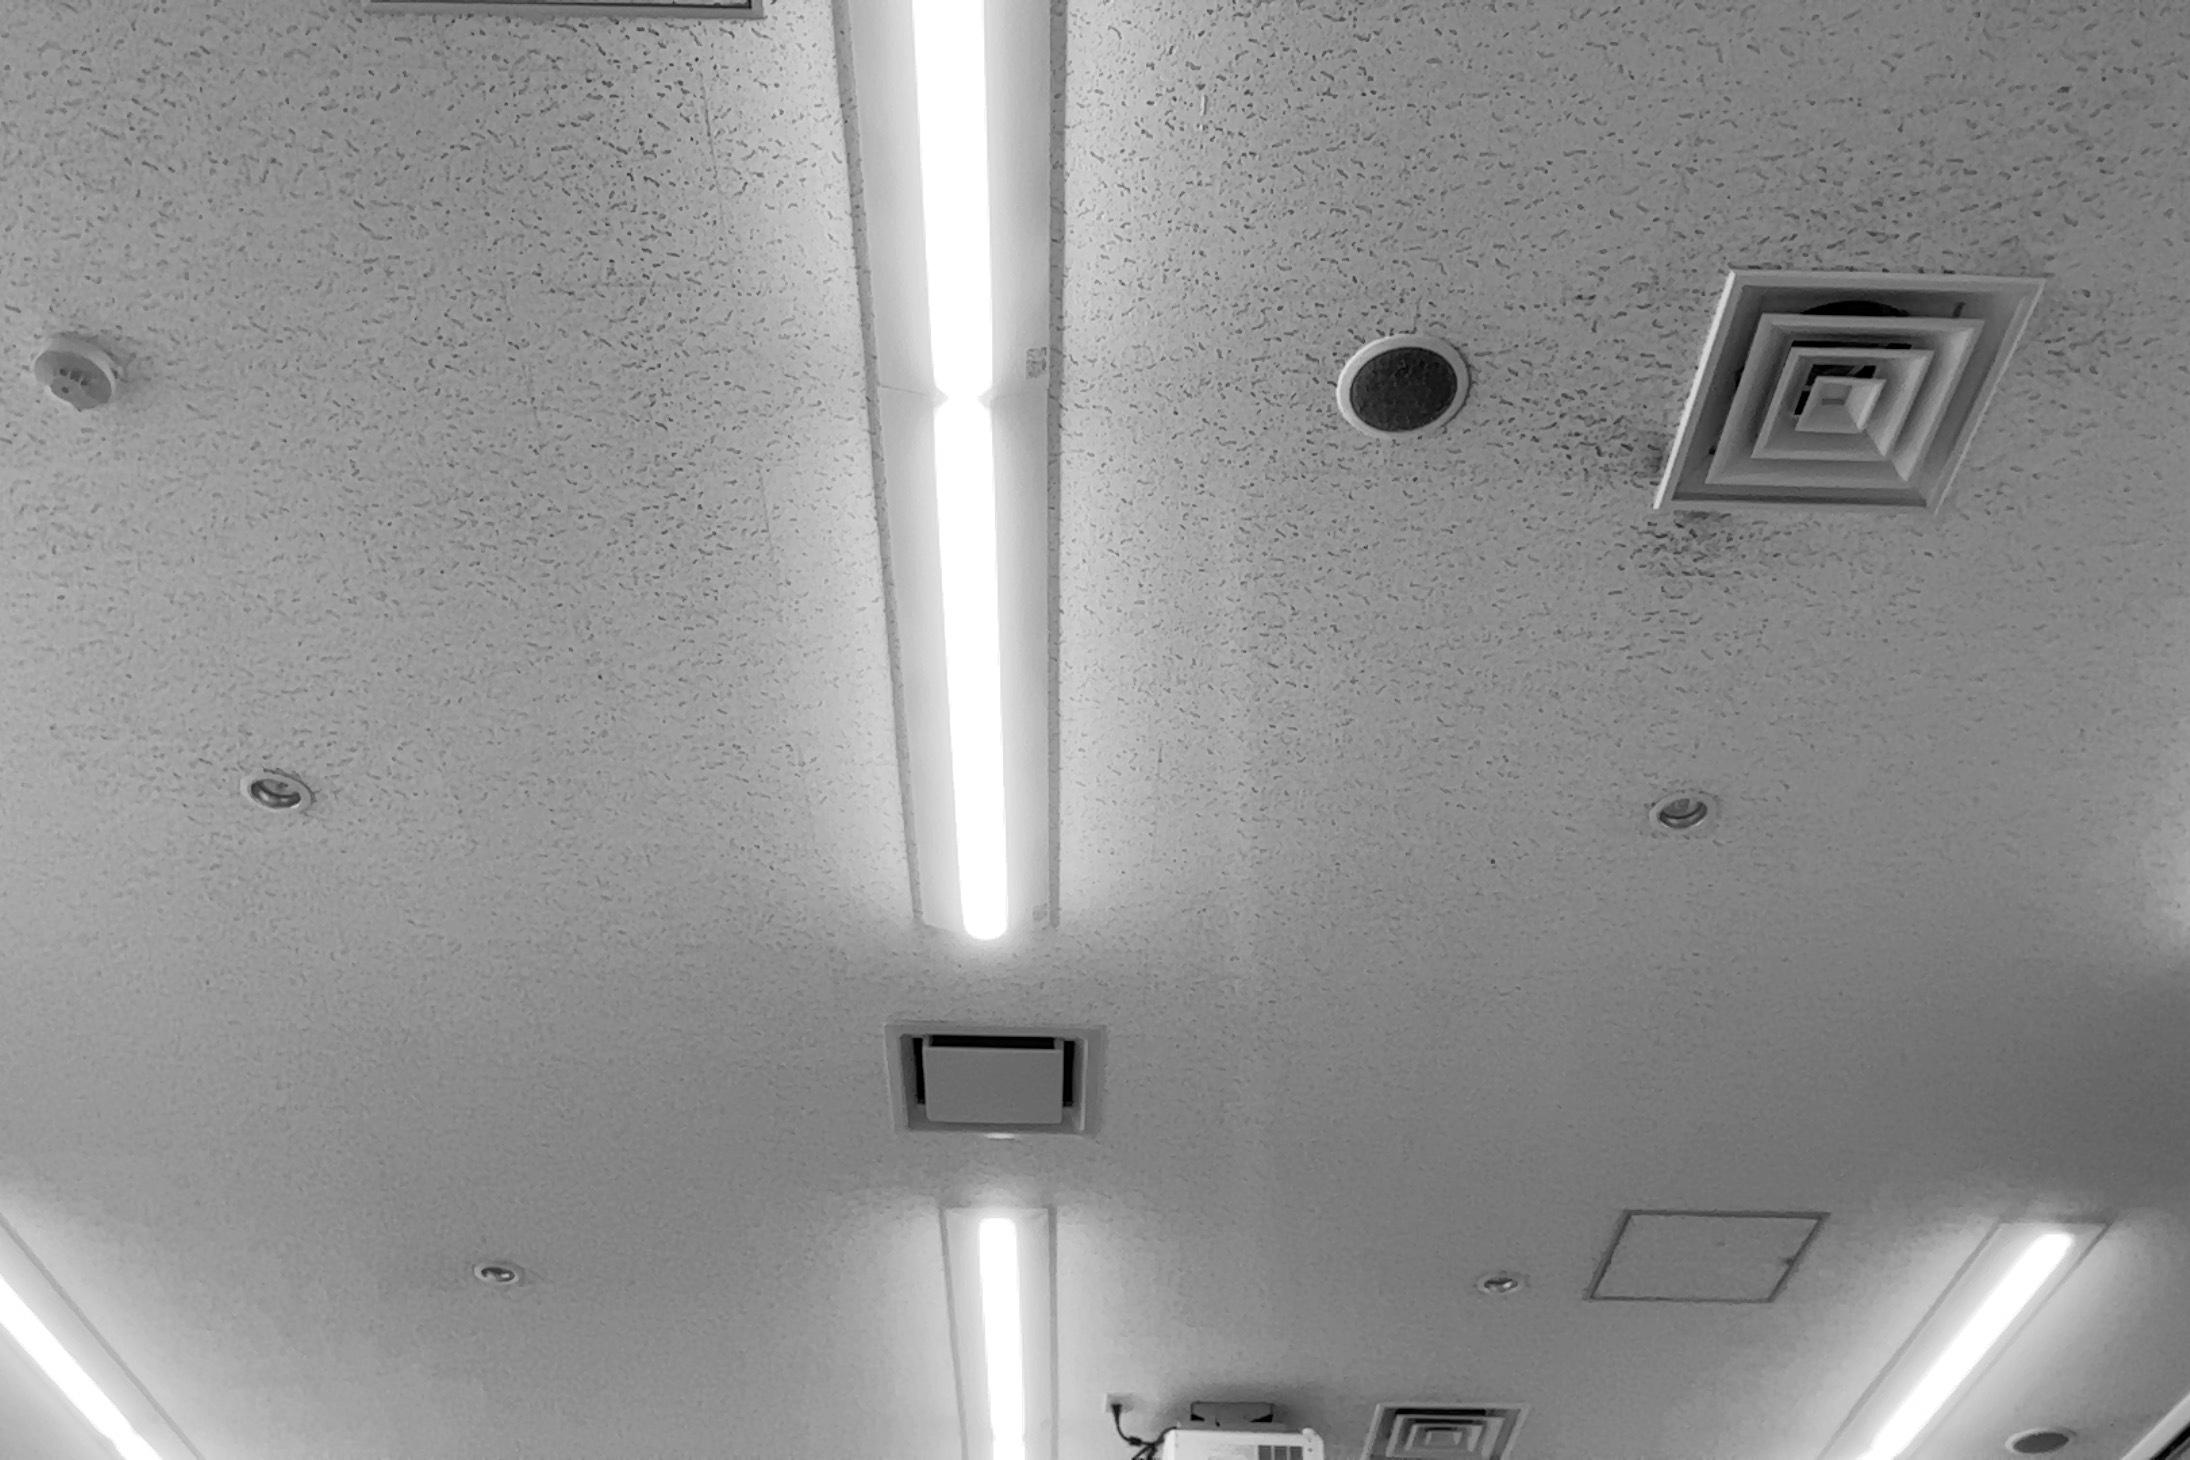
\includegraphics[keepaspectratio,width=\textwidth]{../../05_UnderstandingImages/fig2_g.jpg}
            \subcaption{背景のみ}
        \end{minipage}
        \begin{minipage}[b]{.3\textwidth}
            \centering
            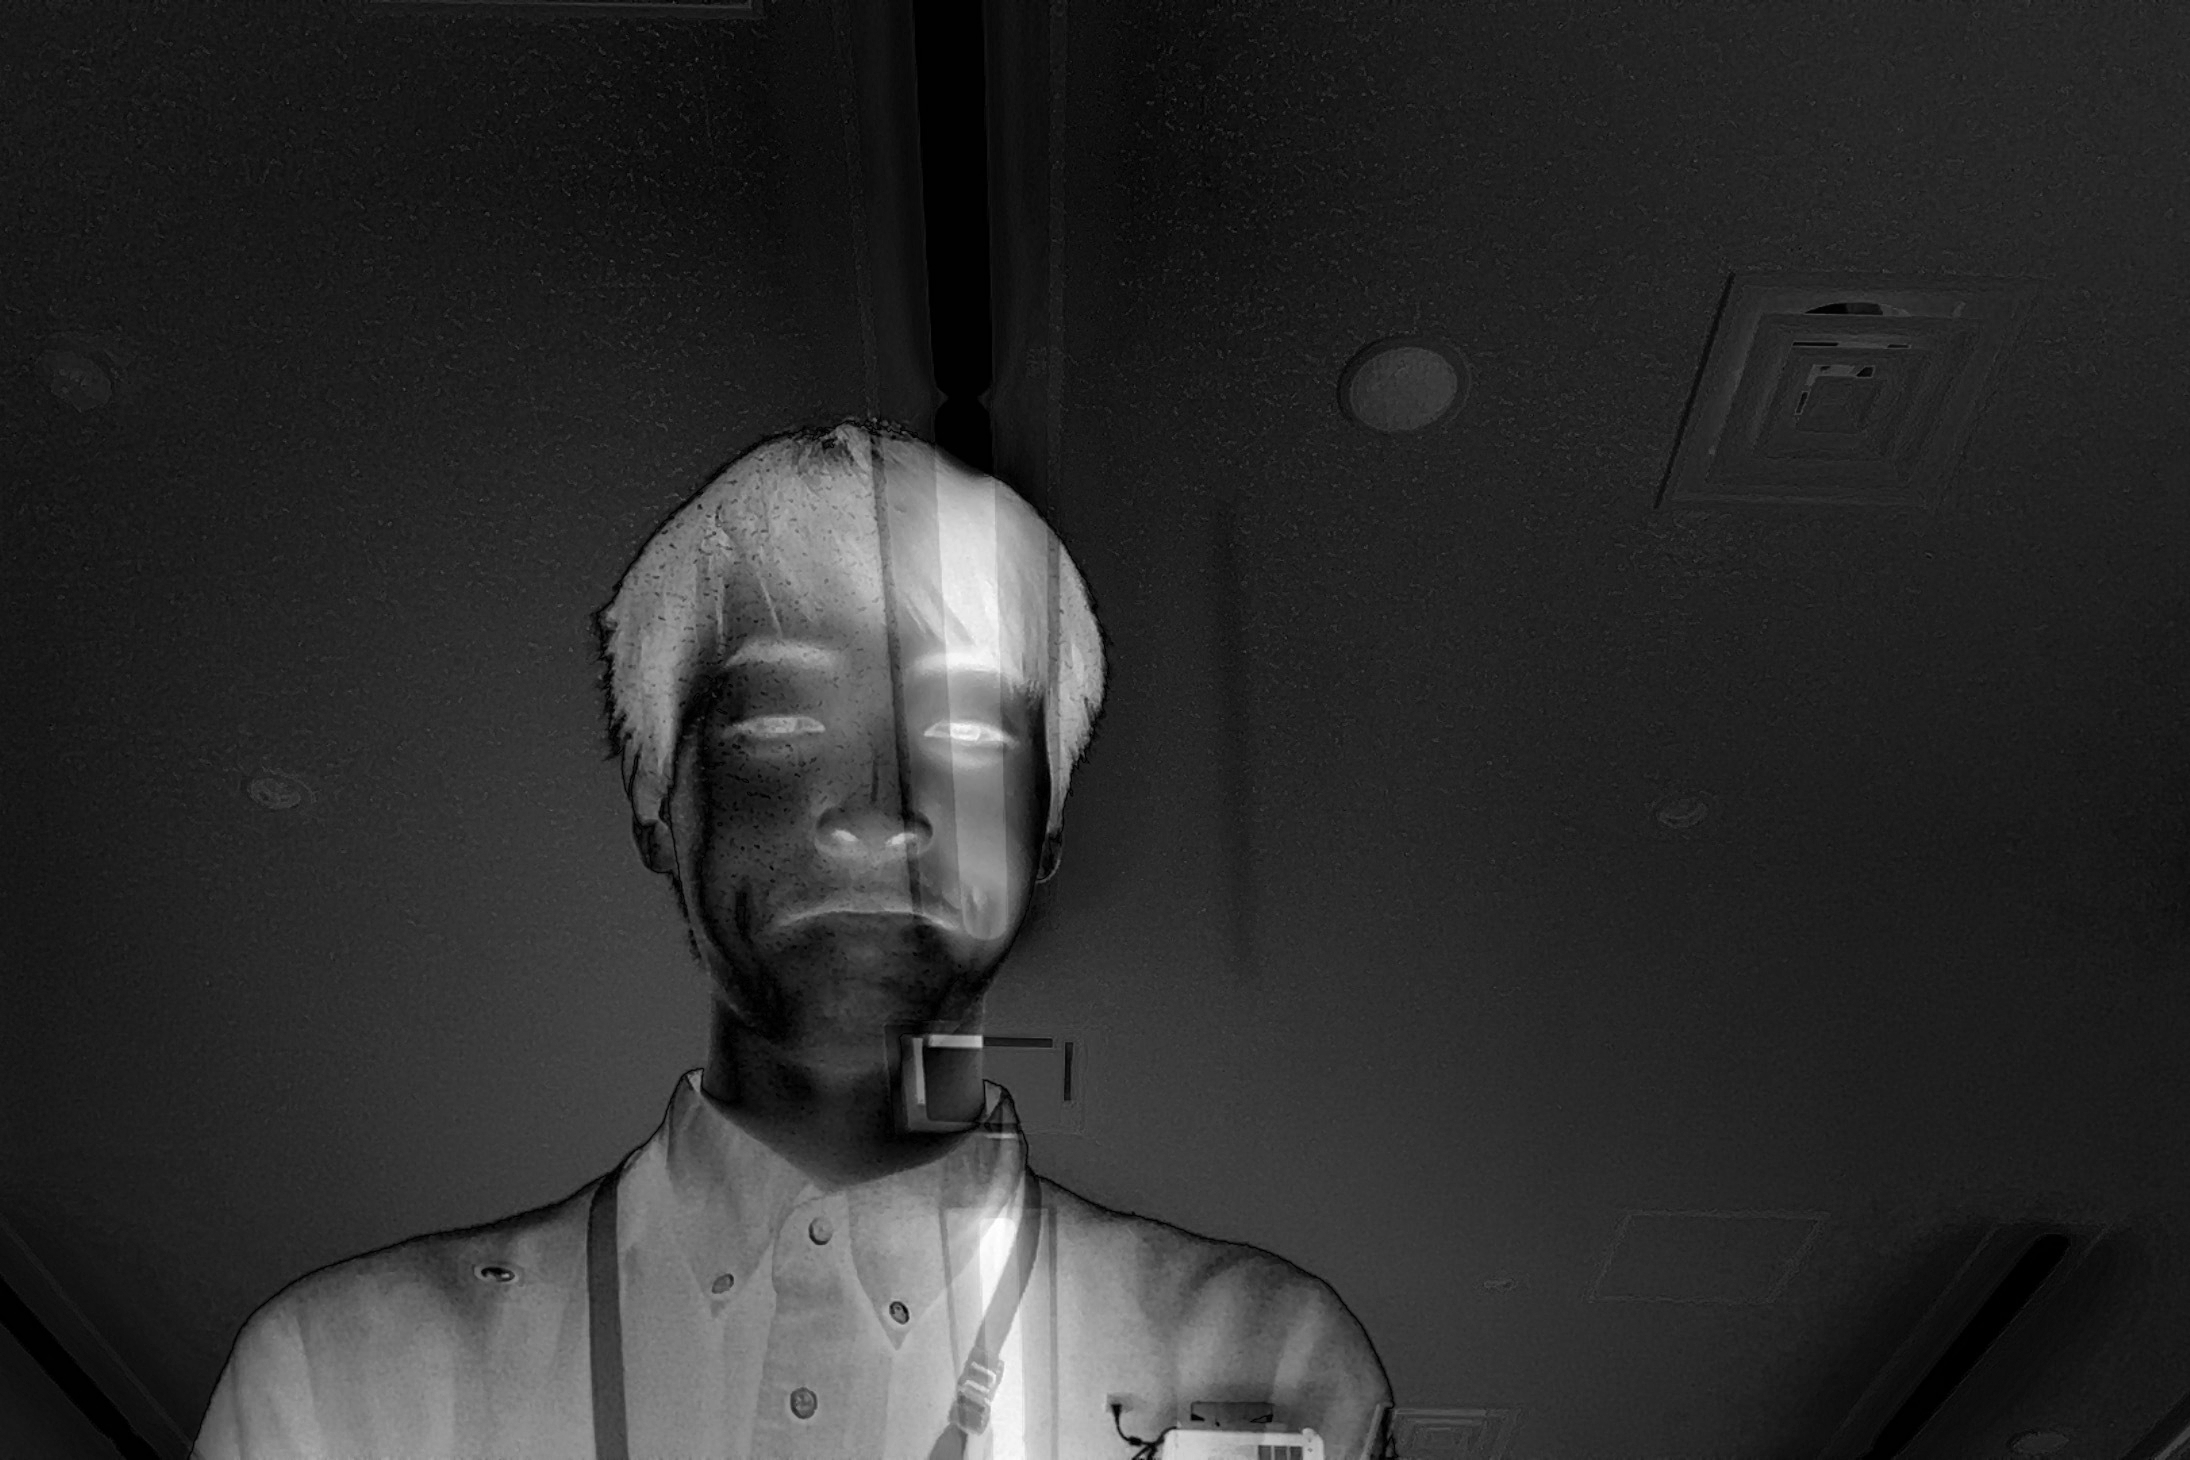
\includegraphics[keepaspectratio,width=\textwidth]{../../Figures/05_60.png}
            \subcaption{背景差分画像}
        \end{minipage}
        \caption{\kadaiaf\ 実験結果}
    \end{minipage}
    \nextfloat
    \begin{minipage}[b]{.49\textwidth}
        \centering
        \begin{minipage}[b]{.3\textwidth}
            \centering
            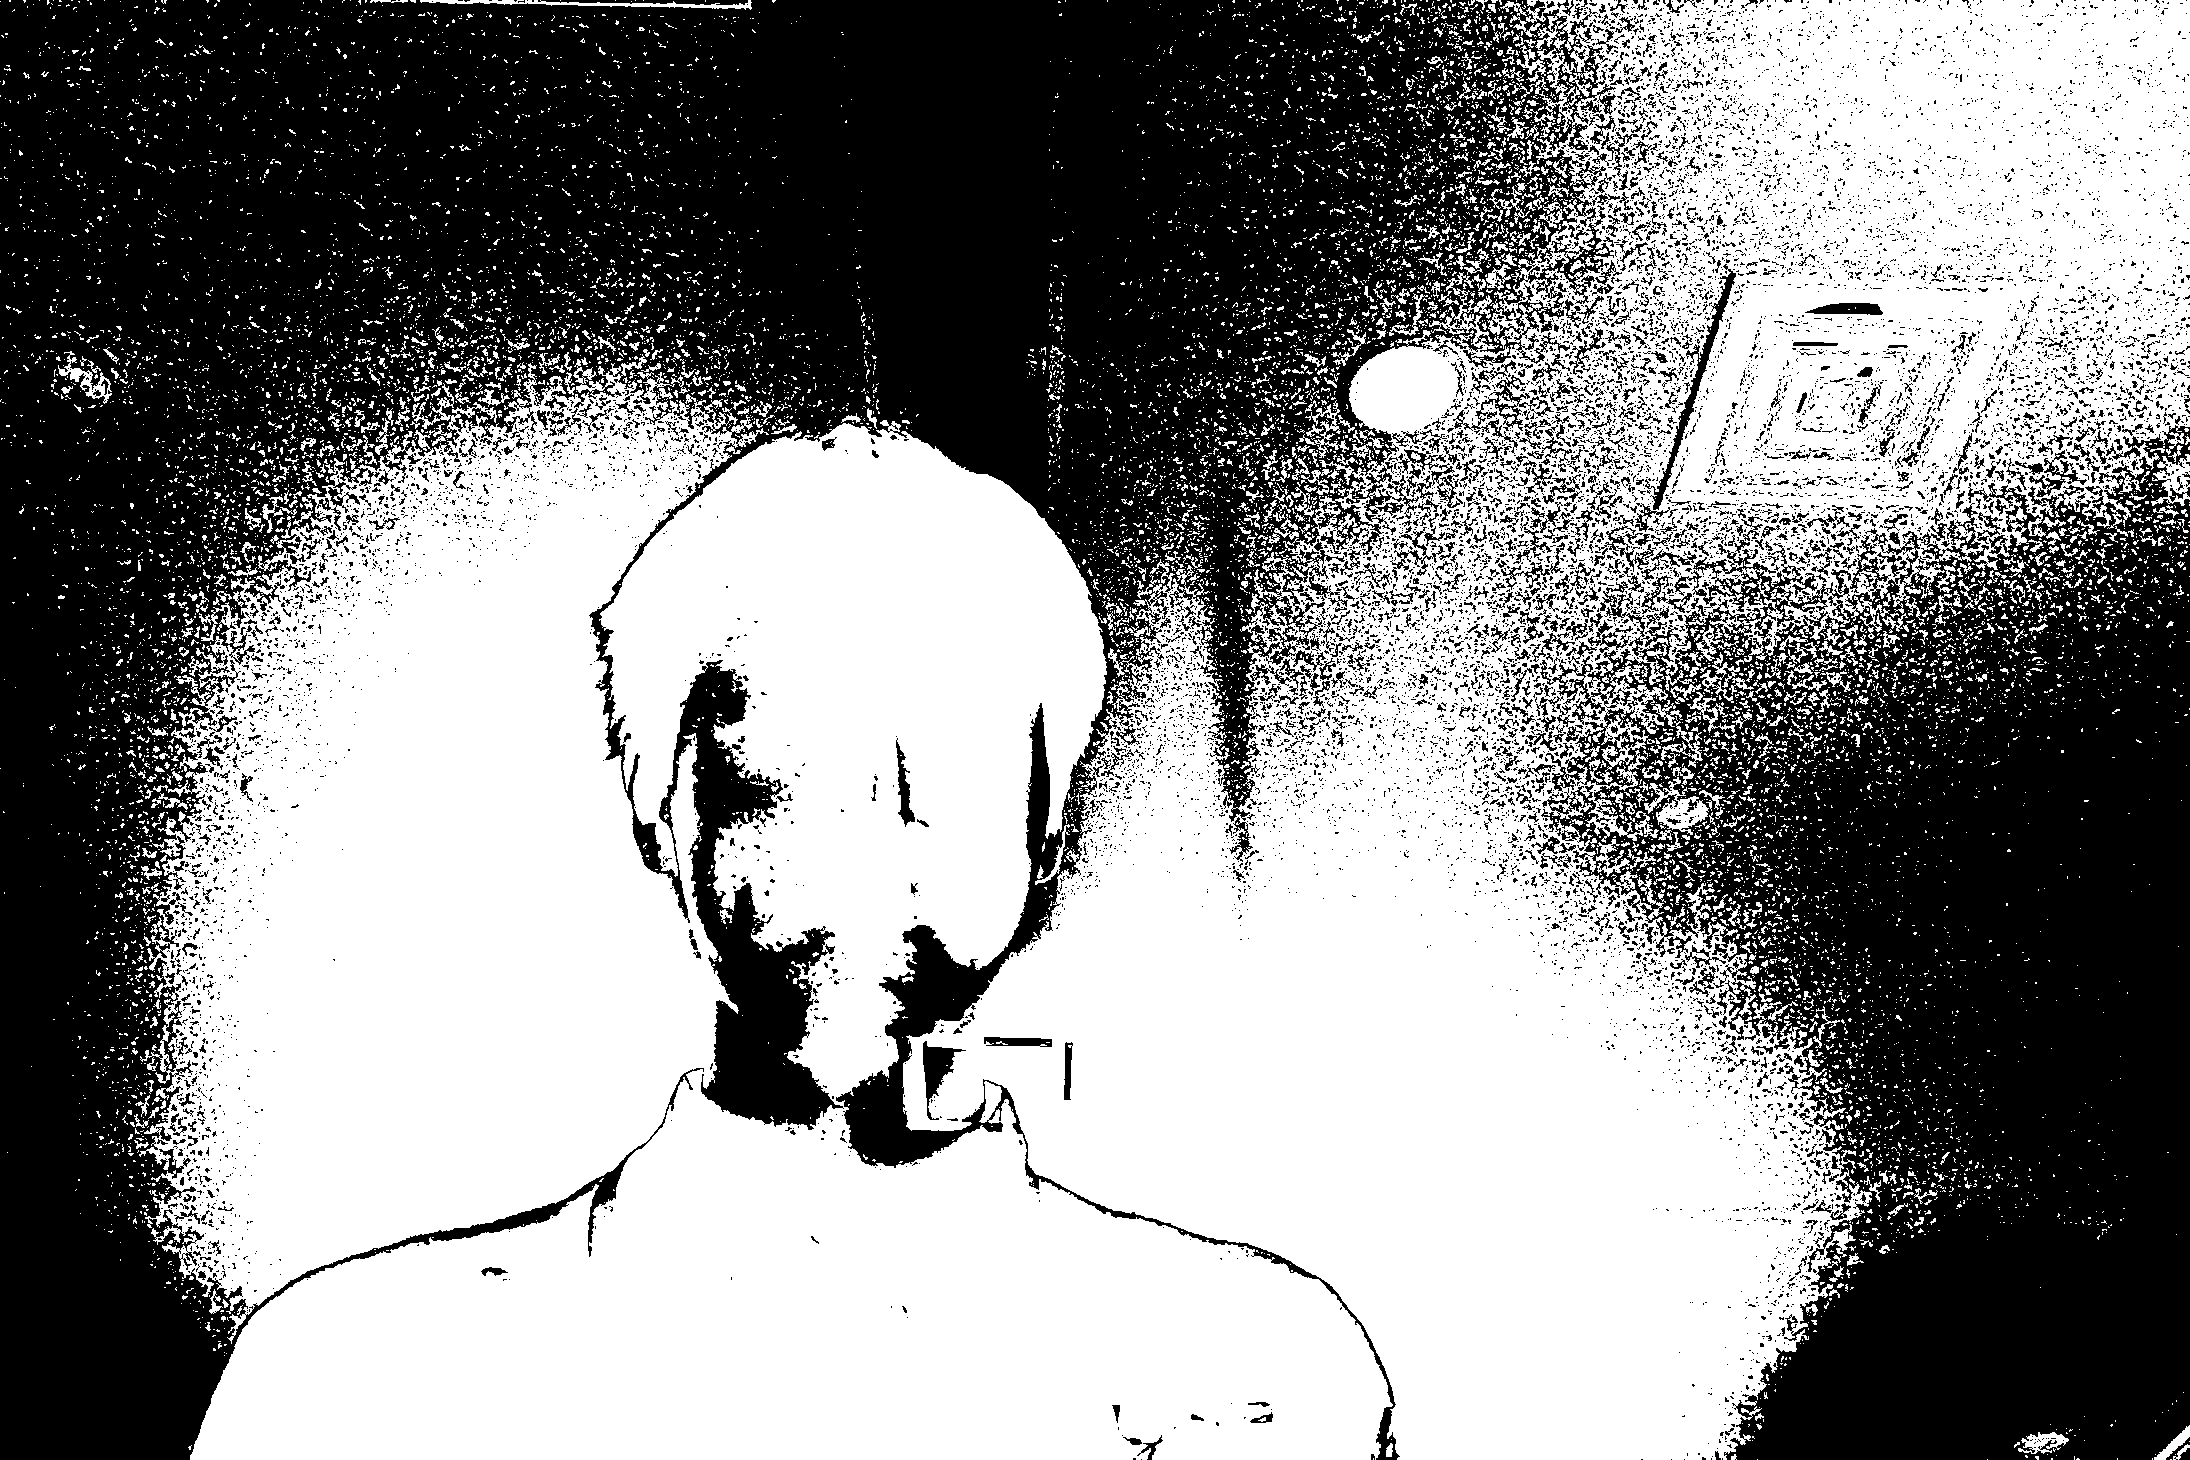
\includegraphics[keepaspectratio,width=\textwidth]{../../Figures/05_61.png}
            \subcaption{閾値\ \(32\)}
        \end{minipage}
        \begin{minipage}[b]{.3\textwidth}
            \centering
            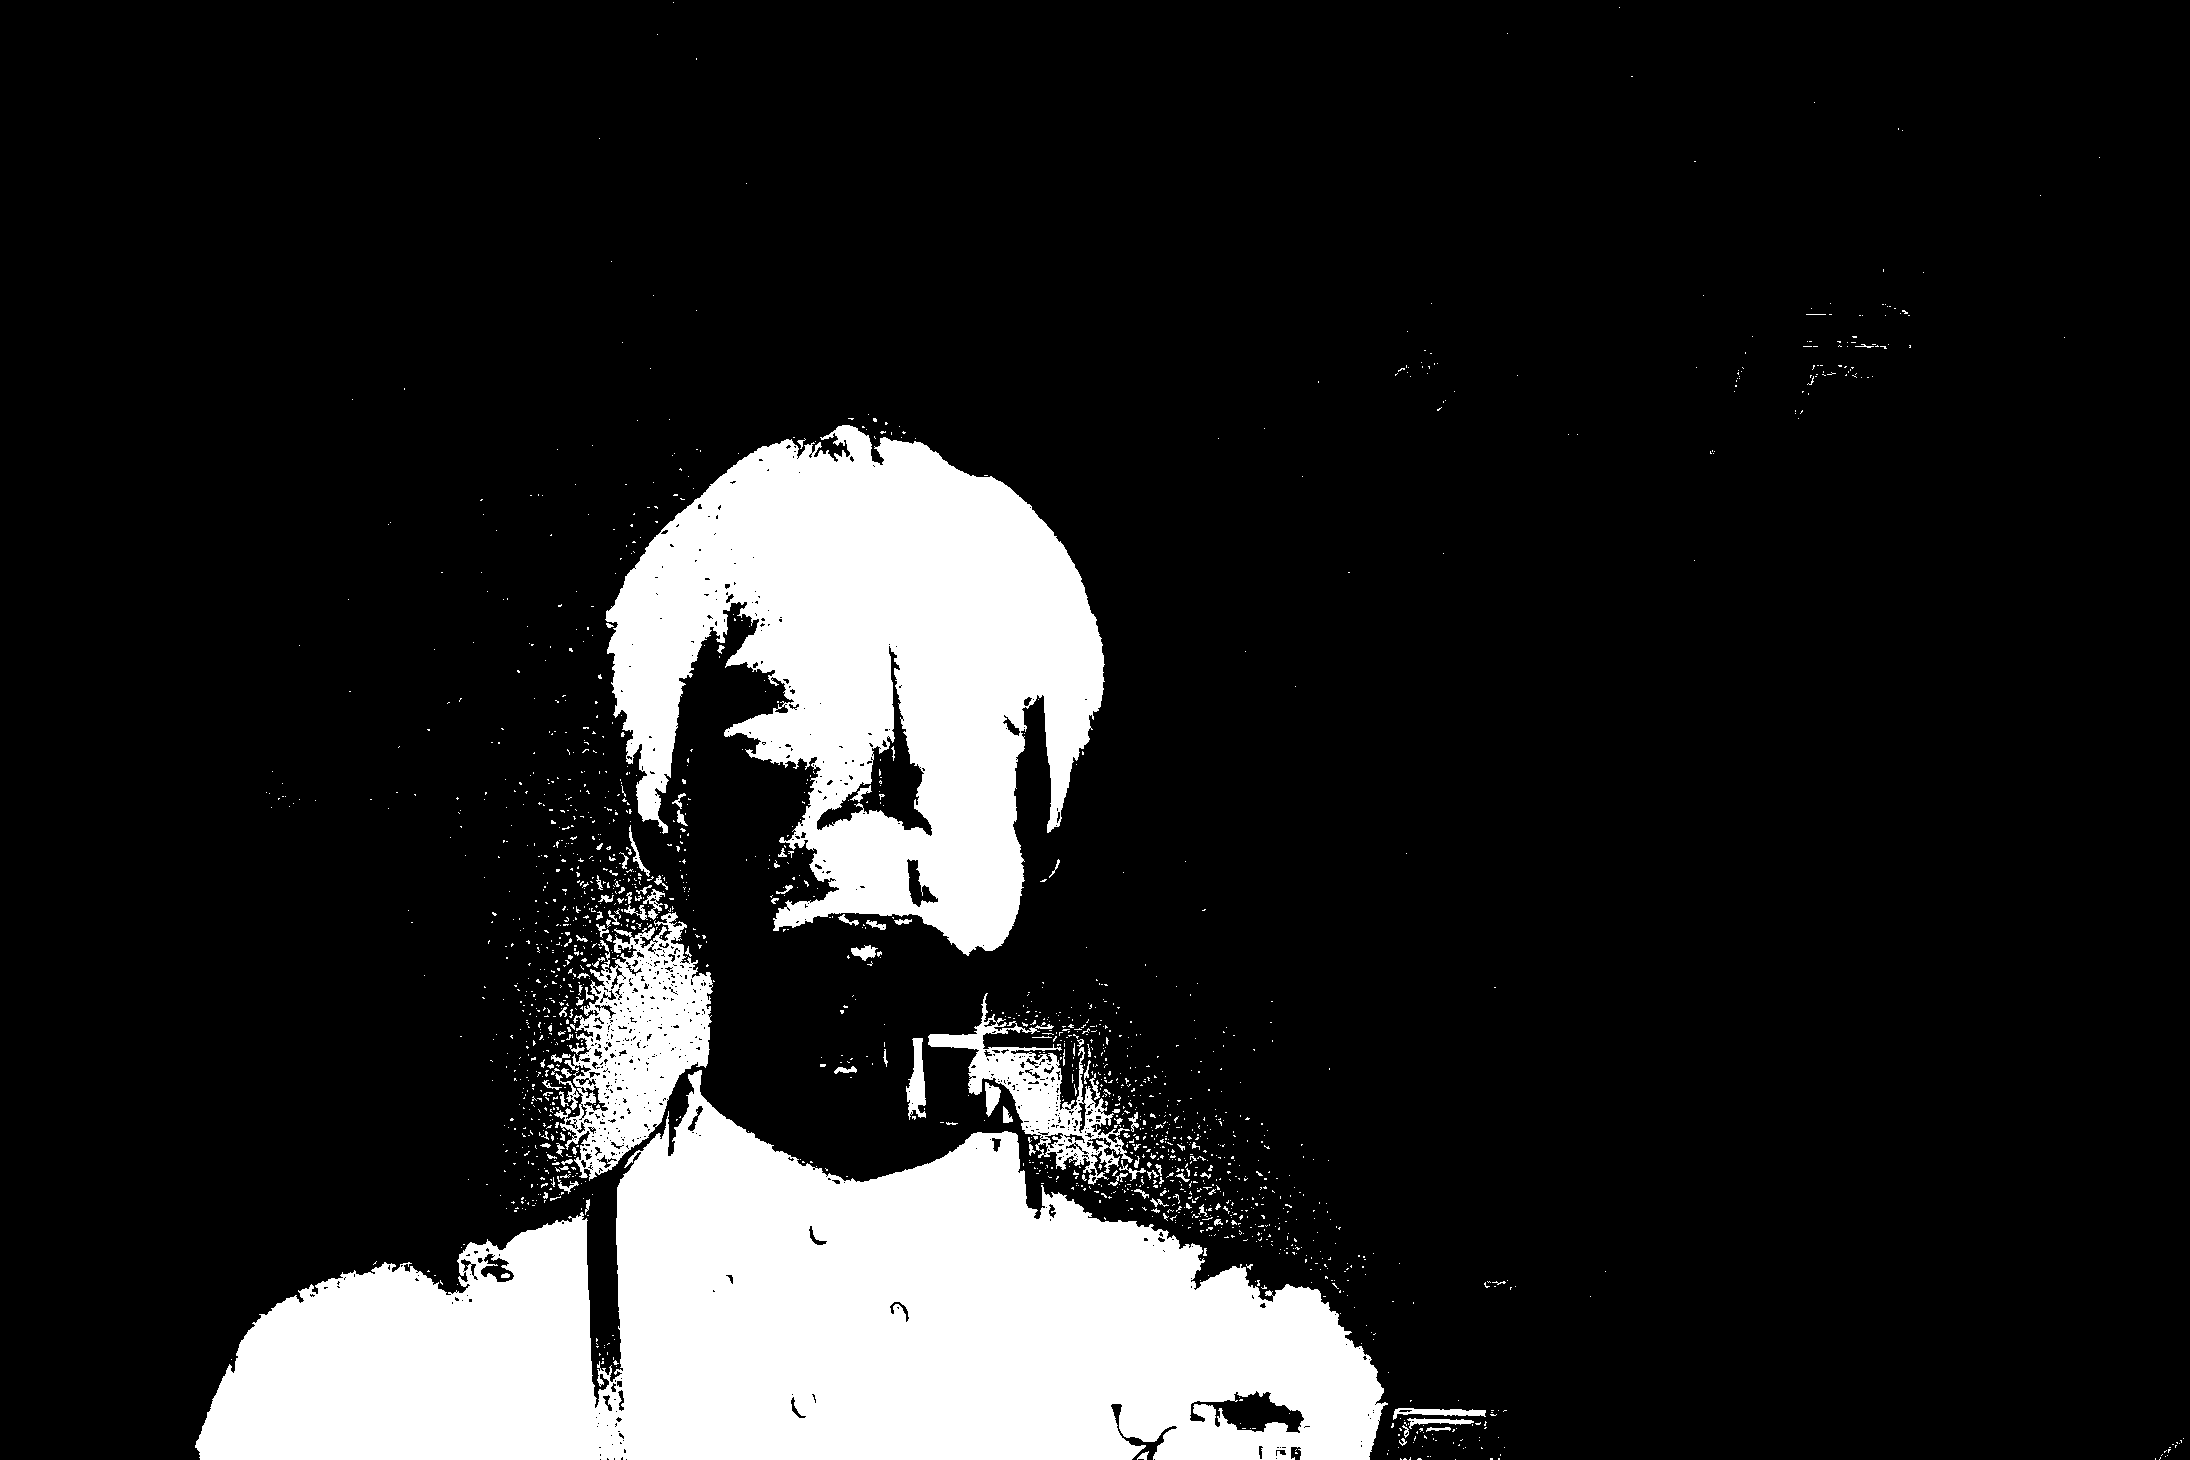
\includegraphics[keepaspectratio,width=\textwidth]{../../Figures/05_62.png}
            \subcaption{閾値\ \(64\)}
        \end{minipage}
        \begin{minipage}[b]{.3\textwidth}
            \centering
            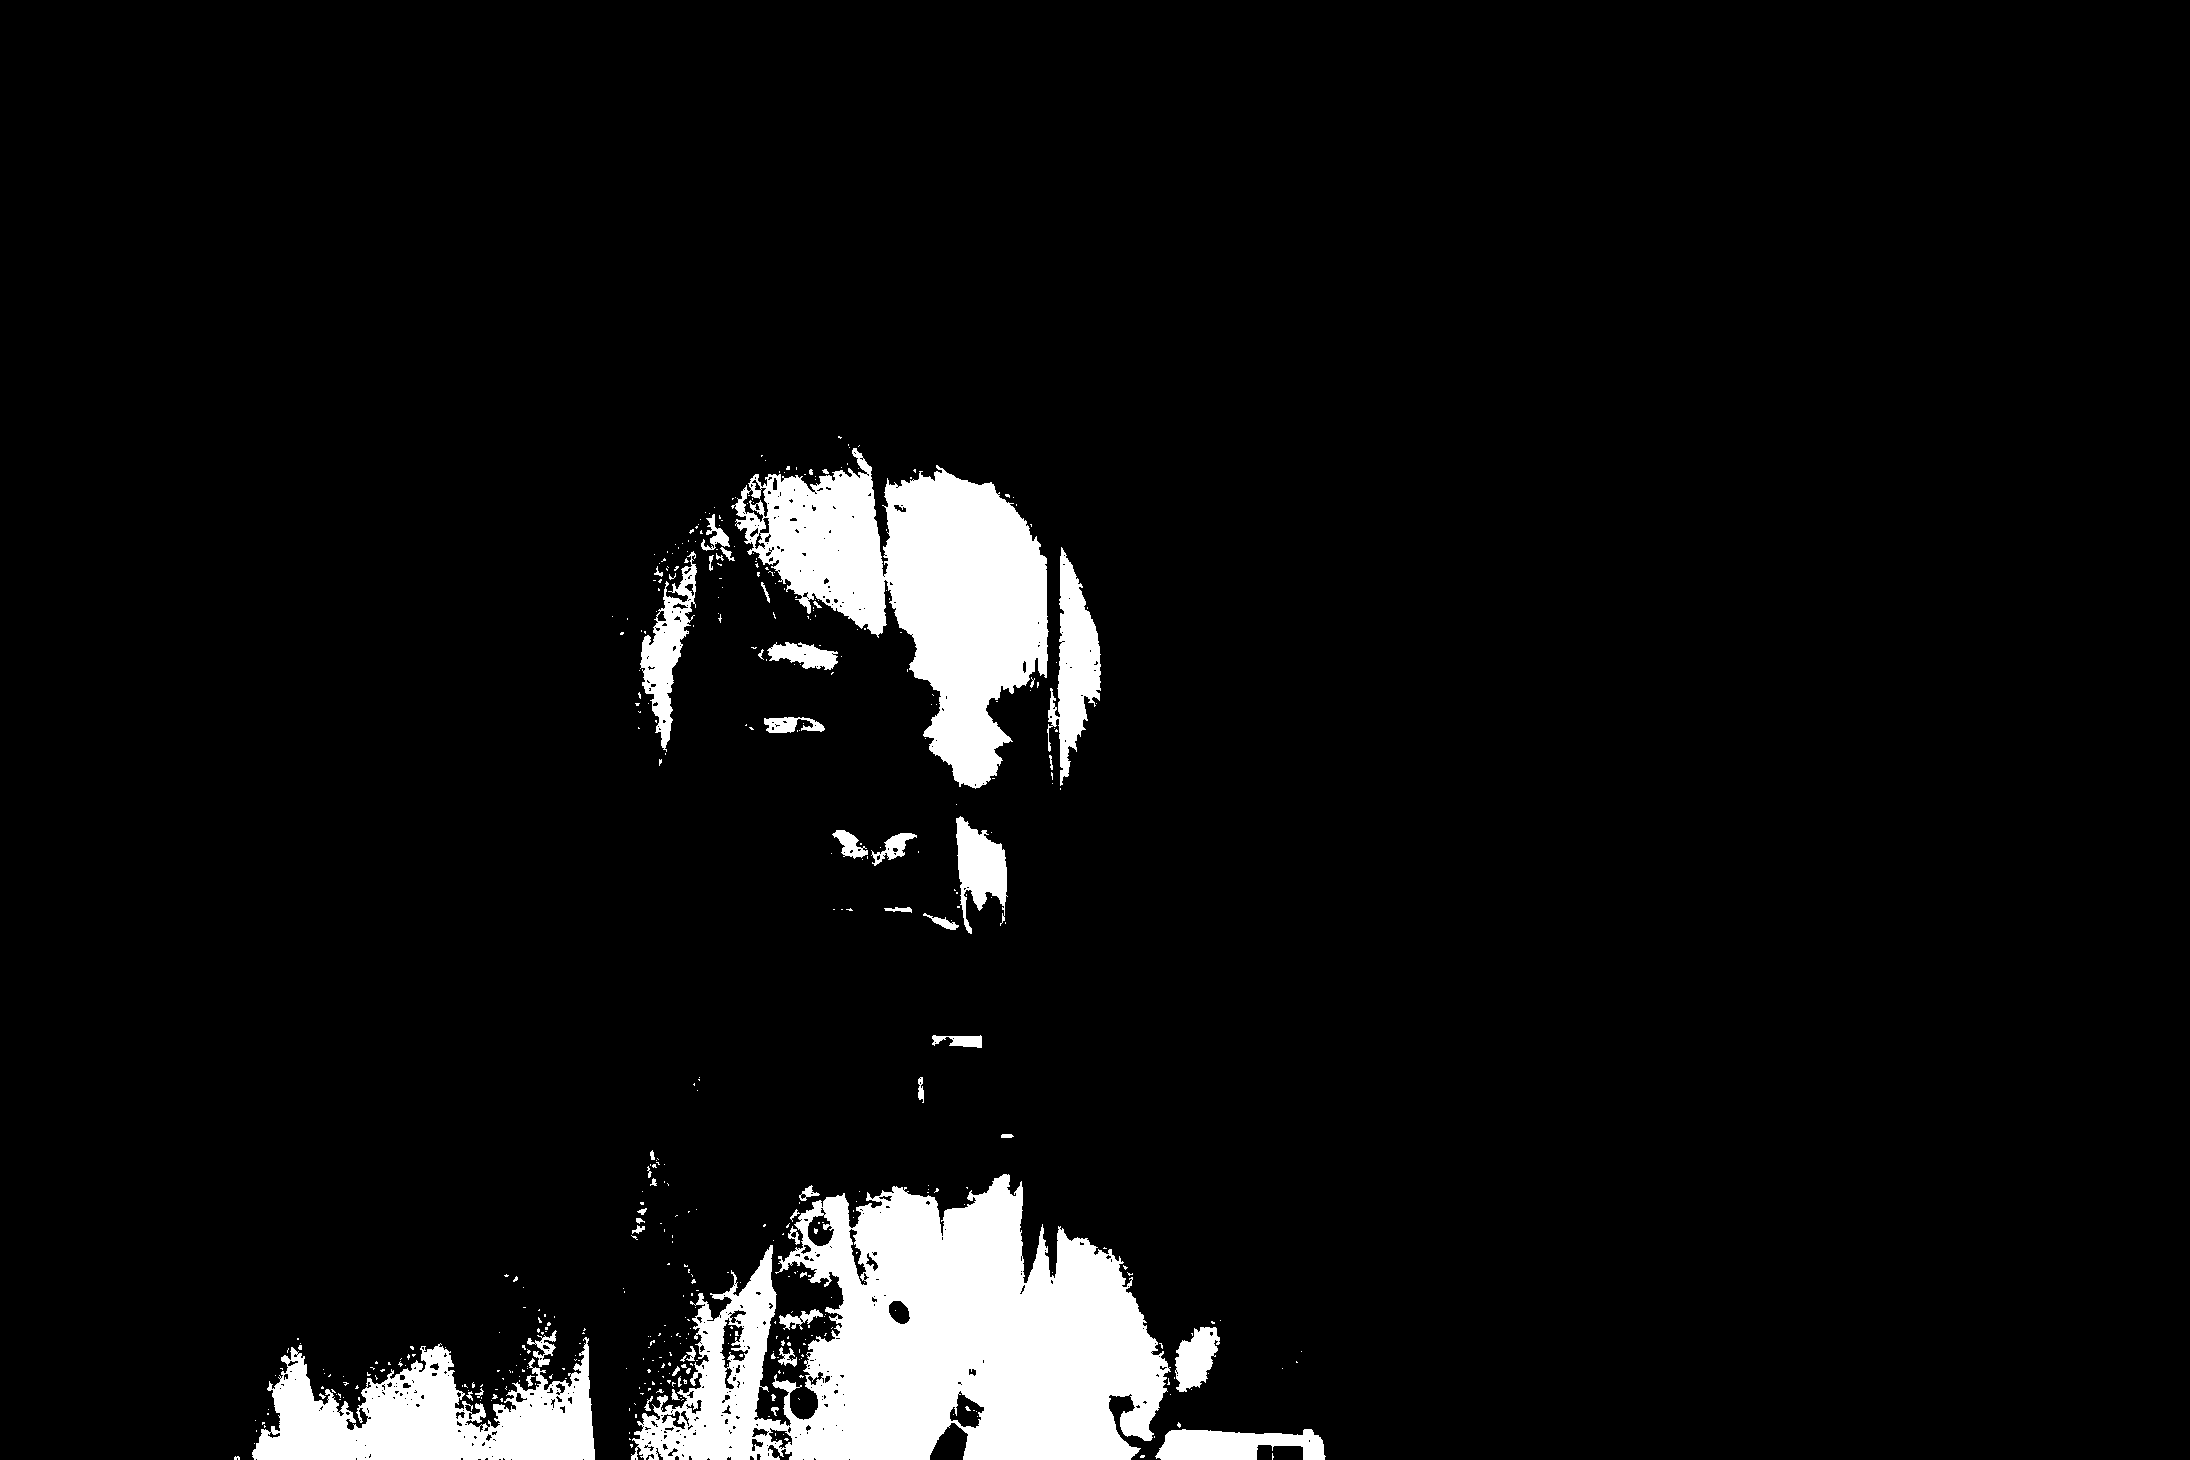
\includegraphics[keepaspectratio,width=\textwidth]{../../Figures/05_63.png}
            \subcaption{閾値\ \(128\)}
        \end{minipage}
        \caption{背景差分画像の閾値処理}
    \end{minipage}
\end{figure}
\footnotetext[1]{NTSC輝度信号のグレイスケール画像}
\begin{figure}[h]
    \centering
    \begin{minipage}[b]{.3\textwidth}
        \centering
        
\includegraphics[keepaspectratio,width=\textwidth]{../../Figures/05_21_gimg.png}
        \subcaption{元画像}
    \end{minipage}
    \begin{minipage}[b]{.3\textwidth}
        \centering
        
\includegraphics[keepaspectratio,width=\textwidth]{../../06_ImageFiltering/file_white-Gaussian-Noise.png}
        \subcaption{白色ガウス雑音(\wgnimg)}
    \end{minipage}
    \begin{minipage}[b]{.3\textwidth}
        \centering
        
\includegraphics[keepaspectratio,width=\textwidth]{../../06_ImageFiltering/file_impluse-noise.png}
        \subcaption{インパルス雑音(\inimg)}
    \end{minipage}
    \caption{\kadaiaa\ 実験結果}
\end{figure}
\paragraph{平滑化フィルタ,メディアンフィルタ}
\wgnimg に対して平滑化フィルタを適用すると,雑音部分が目立たなくなった.また,\inimg に対して平滑化フィルタを適用すると,雑音が取り除かれることなく残った.
\wgnimg と\inimg に対してメディアンフィルタを適用すると,雑音部分が目立たなくなった.
\begin{figure}[H]
    \centering
    \begin{minipage}[b]{.49\textwidth}
        \begin{minipage}[b]{.49\textwidth}
            
\includegraphics[keepaspectratio,width=\textwidth]{../../Figures/06_21_sf_img_wgn.png}
            \subcaption{\wgnimg}
        \end{minipage}
        \begin{minipage}[b]{.49\textwidth}
            
\includegraphics[keepaspectratio,width=\textwidth]{../../Figures/06_22_sf_img_in.png}
            \subcaption{\inimg}
        \end{minipage}
        \caption{平滑化フィルタ}
    \end{minipage}
    \begin{minipage}[b]{.49\textwidth}
        \begin{minipage}[b]{.49\textwidth}
            
\includegraphics[keepaspectratio,width=\textwidth]{../../Figures/06_23_mf_img_wgn.png}
            \subcaption{\wgnimg}
        \end{minipage}
        \begin{minipage}[b]{.49\textwidth}
            
\includegraphics[keepaspectratio,width=\textwidth]{../../Figures/06_24_mf_img_in.png}
            \subcaption{\inimg}
        \end{minipage}
        \caption{メディアンフィルタ}
    \end{minipage}
\end{figure}
\paragraph{Sobelフィルタ,Laplacianフィルタ}
横微分フィルタを適用すると,縦方向のエッジが強調され,縦方向微分フィルタを適用すると,横方向のエッジが強調された.
これらの画像を足し合わせて,\(255\)を上回る値を処理すると,画像全体のエッジが強調された画像を生成できた.
Laplacianフィルタを適用すると,画像が暗く出力された.この画像に対して\figref{fig:Laplacianフィルタのヒストグラム}を用いて,閾値\(30\)の閾値処理し,全体画像のエッジが強調された画像を生成できた.
\begin{figure}[H]
    \centering
    \begin{minipage}[b]{.3\textwidth}
        \centering
        
\includegraphics[keepaspectratio,width=\textwidth]{../../Figures/06_31_diff-x-img.png}
        \subcaption{横方向Sobelフィルタ}
    \end{minipage}
    \begin{minipage}[b]{.3\textwidth}
        \centering
        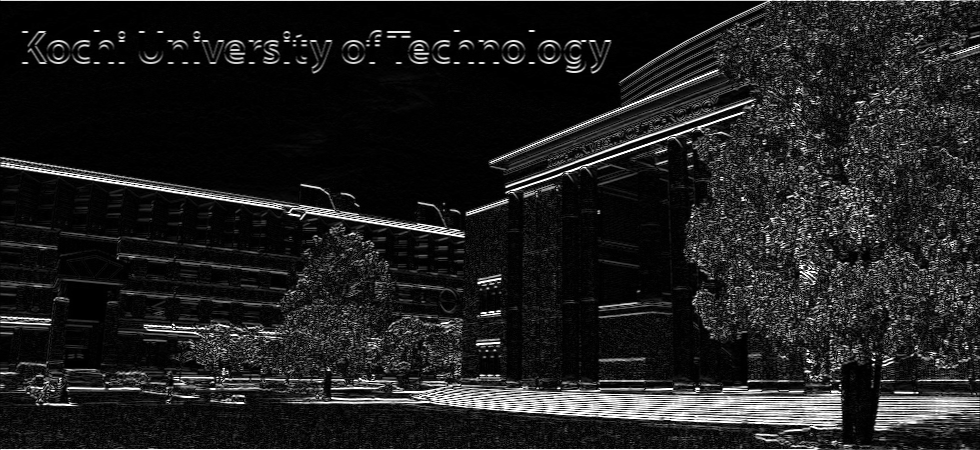
\includegraphics[keepaspectratio,width=\textwidth]{../../Figures/06_32_diff-y-img.png}
        \subcaption{縦方向Sobelフィルタ}
    \end{minipage}
    \begin{minipage}[b]{.3\textwidth}
        \centering
        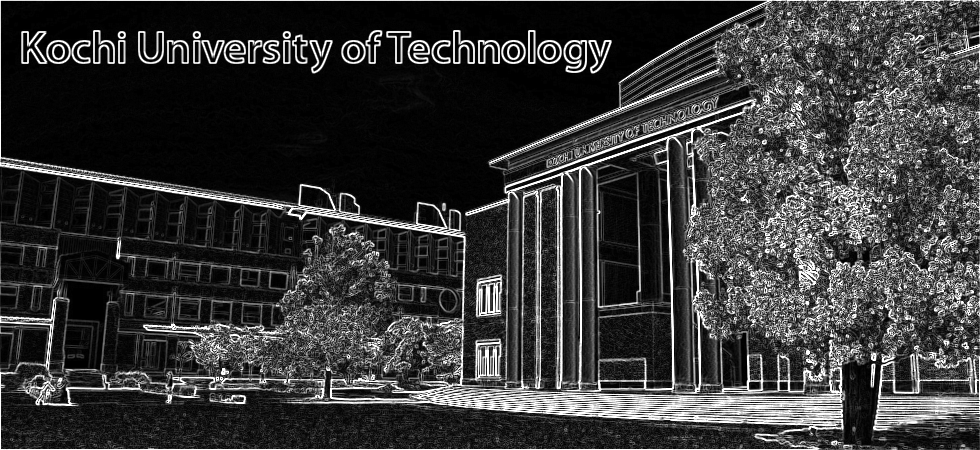
\includegraphics[keepaspectratio,width=\textwidth]{../../Figures/06_33_diff-img.png}
        \subcaption{Sobelフィルタ\footnotemark}
    \end{minipage}
    \caption{Sobelフィルタ適用}
\end{figure}
\begin{figure}[H]
    \centering
    \begin{minipage}[b]{.3\textwidth}
        \centering
        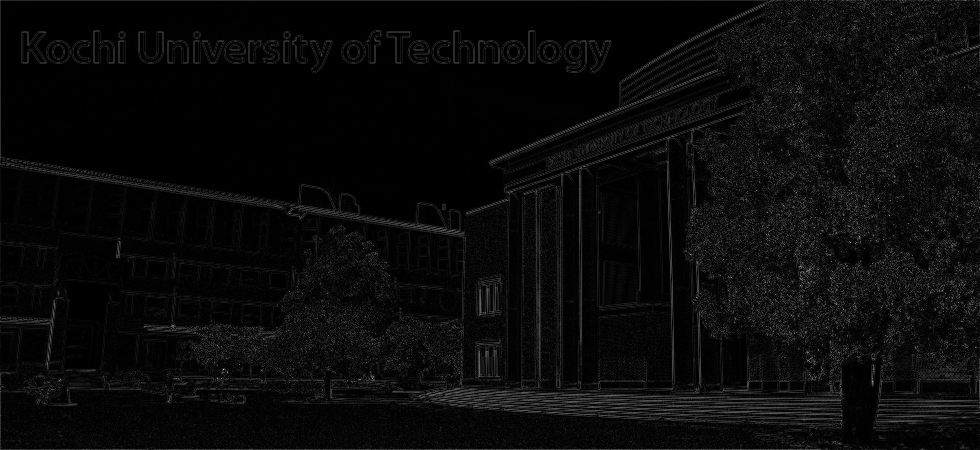
\includegraphics[keepaspectratio,width=\textwidth]{../../Figures/06_41_lf-img}
        \subcaption{Laplacianフィルタ}
    \end{minipage}
    \begin{minipage}[b]{.3\textwidth}
        \centering
        
\includegraphics[keepaspectratio,width=\textwidth]{../../Figures/06_43_lf-img-thresholding.png}
        \subcaption{閾値処理\ \((=30)\)}
    \end{minipage}
    \begin{minipage}[b]{.3\textwidth}
        \centering
        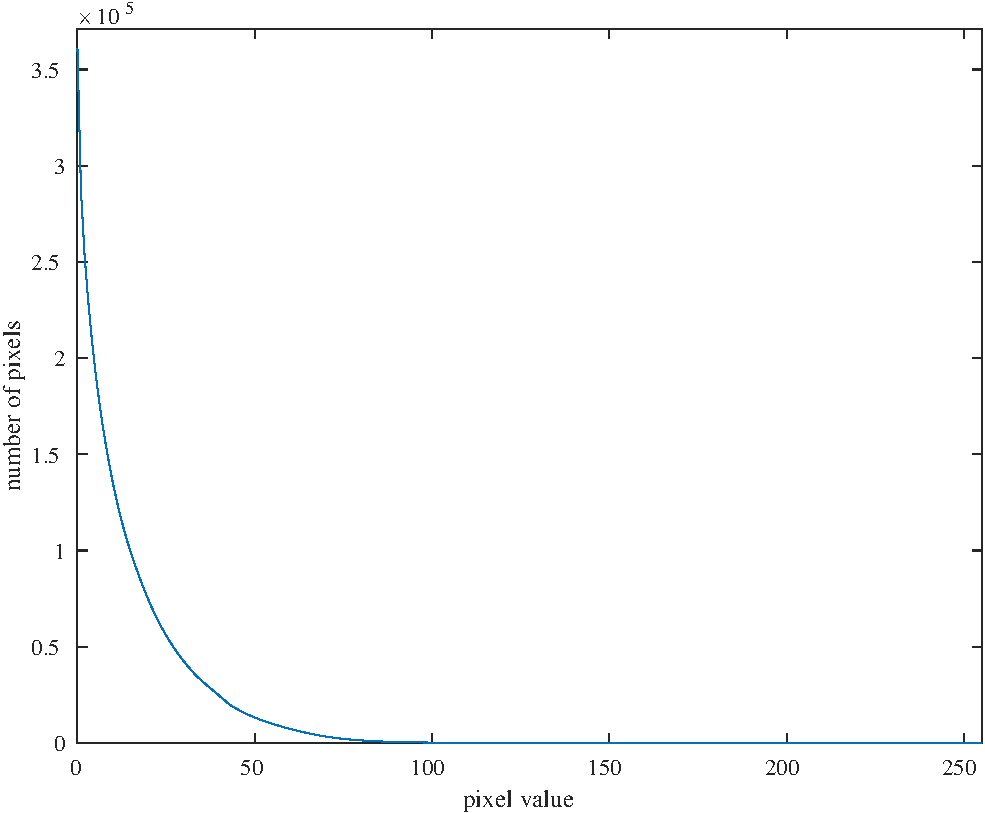
\includegraphics[keepaspectratio,width=\textwidth]{../../Figures/06_42_Thresholding-graph.pdf}
        \subcaption{画素値ヒストグラム}
        \label{fig:Laplacianフィルタのヒストグラム}
    \end{minipage}
    \caption{Laplacianフィルタの適用と処理}
\end{figure}
\footnotetext[1]{横方向Sobelフィルタ適用後画像と縦方向Sobelフィルタ適用後画像の和.}
\begin{figure}[H]
    \centering
    \begin{minipage}[b]{.23\textwidth}
        \centering
        \includegraphics[keepaspectratio,width=\textwidth]{../../06_ImageFiltering/file_hand.png}
        \subcaption{元画像}
    \end{minipage}
    \begin{minipage}[b]{.23\textwidth}
        \centering
        \includegraphics[keepaspectratio,width=\textwidth]{../../Figures/06_51_img-hsv.png}
        \subcaption{HSV色空間への変換後}
    \end{minipage}
    \begin{minipage}[b]{.23\textwidth}
        \centering
        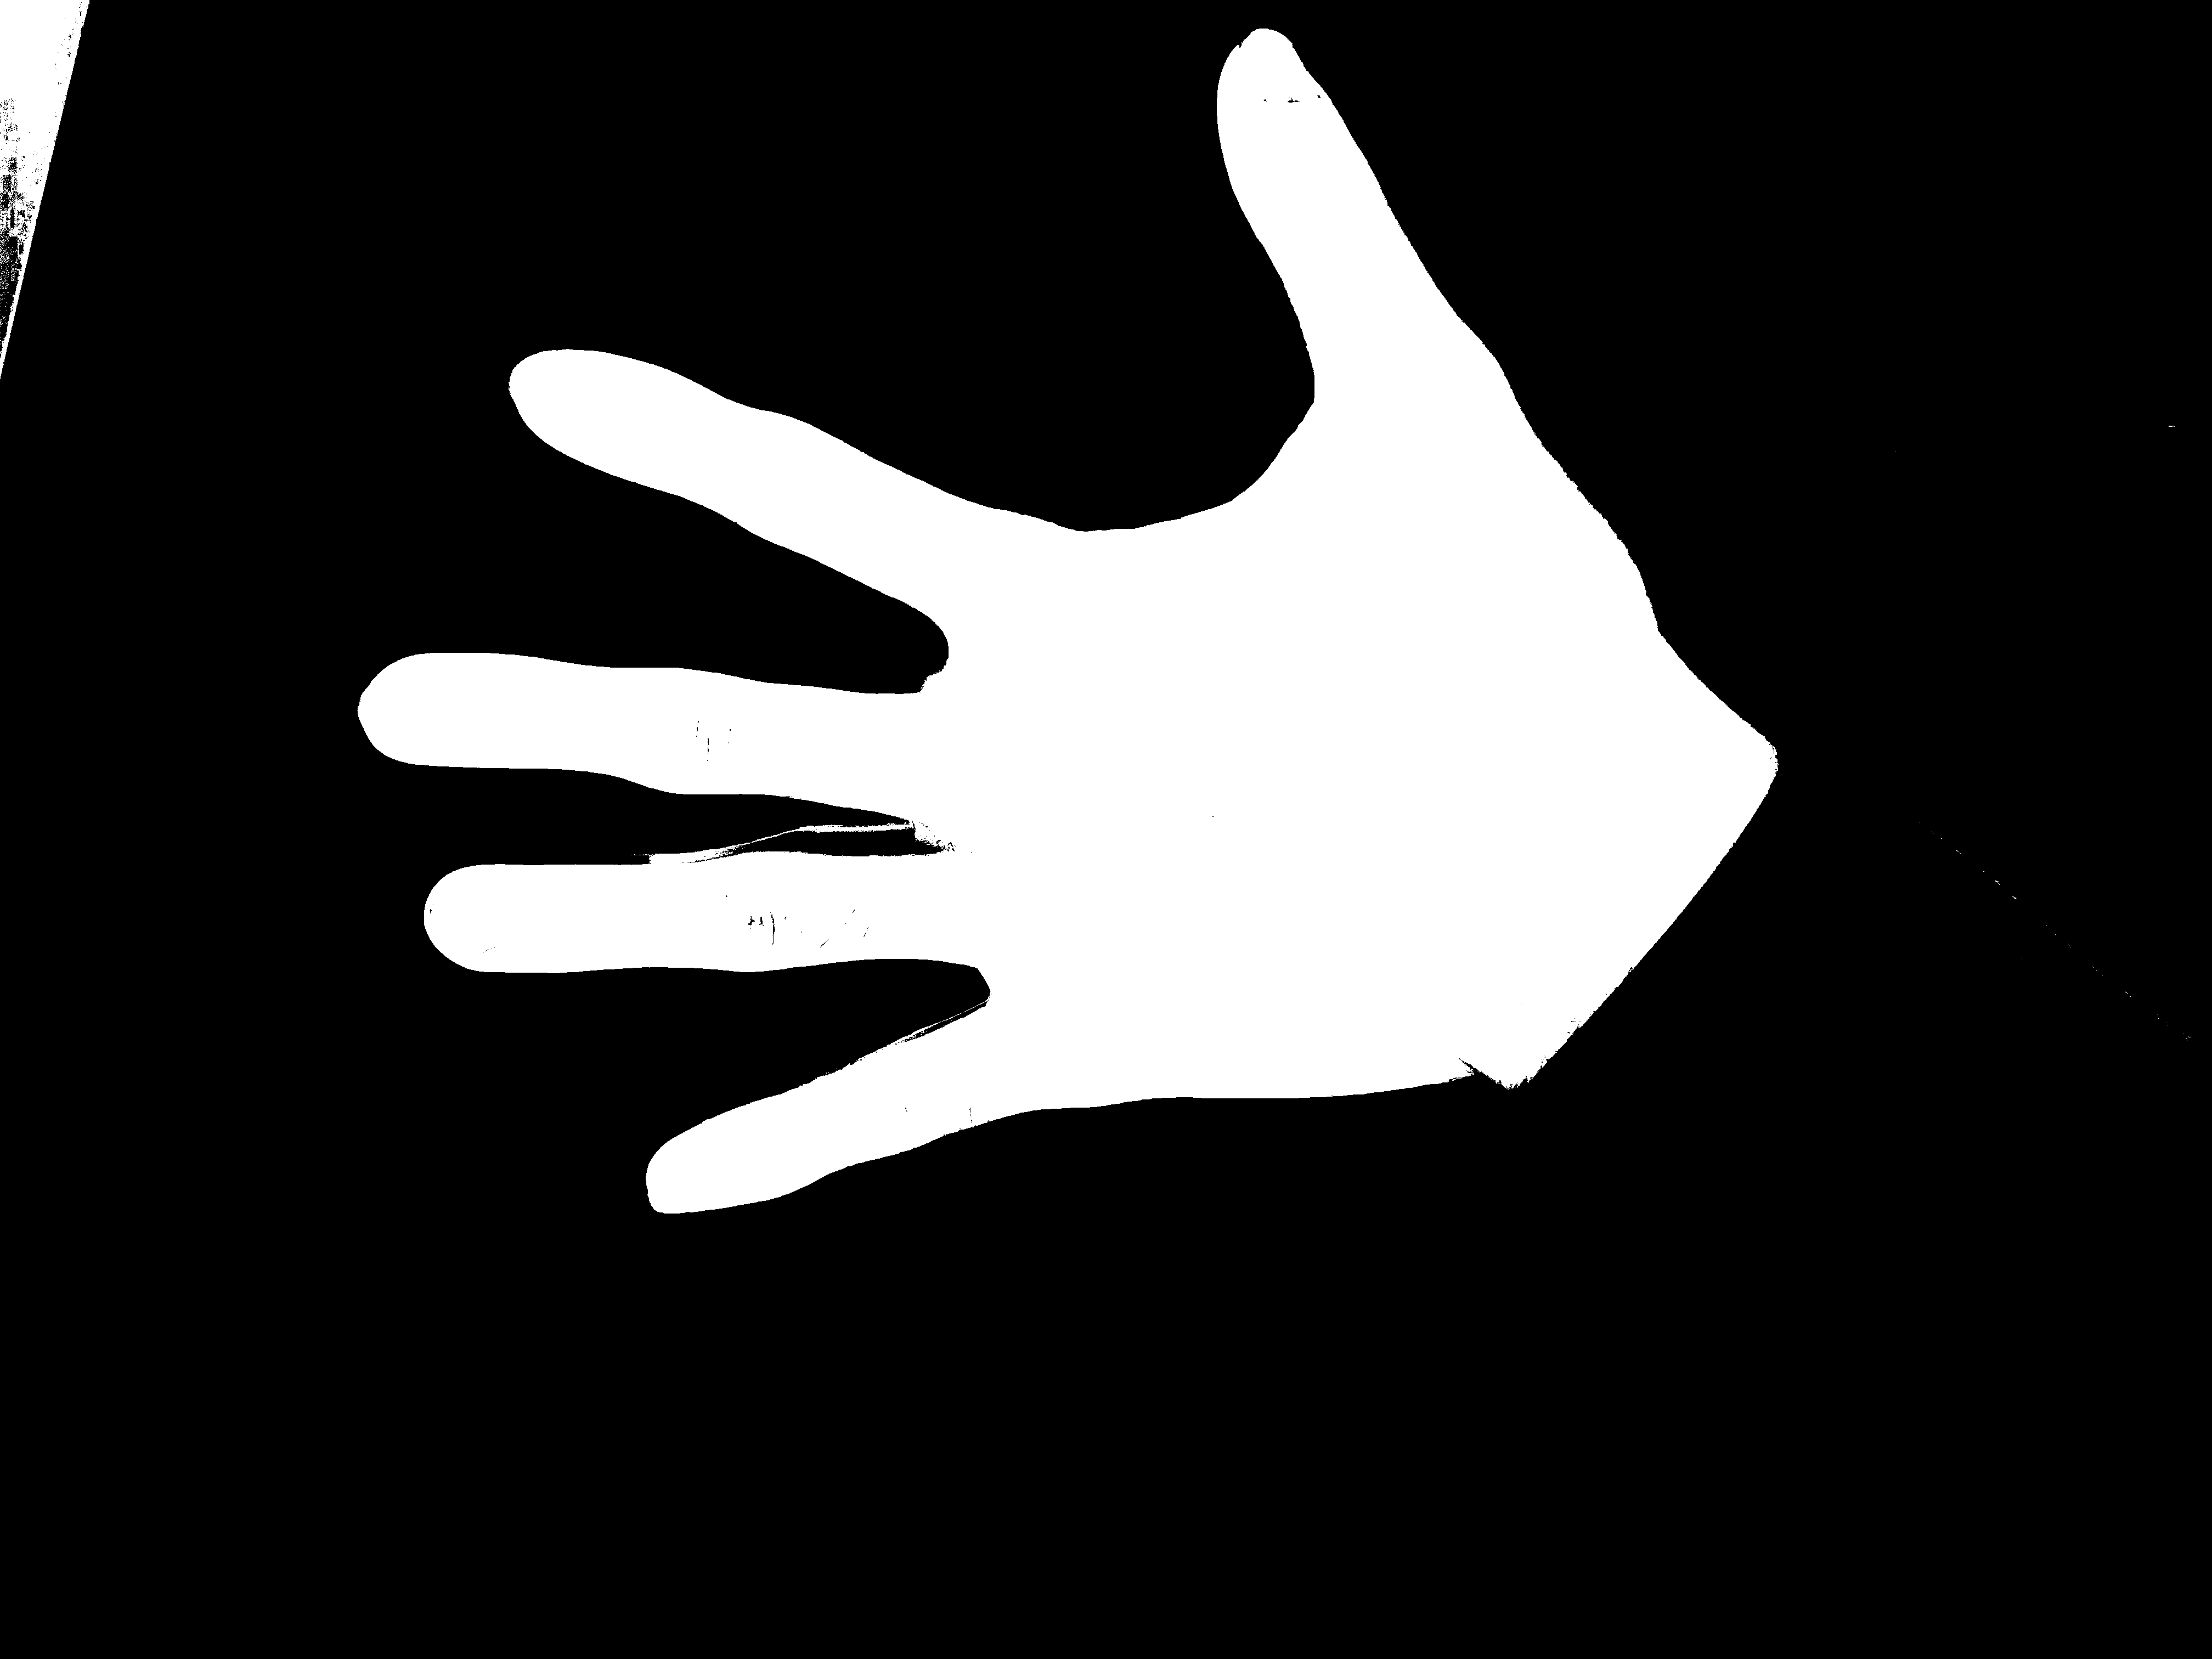
\includegraphics[keepaspectratio,width=\textwidth]{../../Figures/06_52_scd.png}
        \subcaption{肌色領域の抽出(HSV)}
    \end{minipage}
    \begin{minipage}[b]{.23\textwidth}
        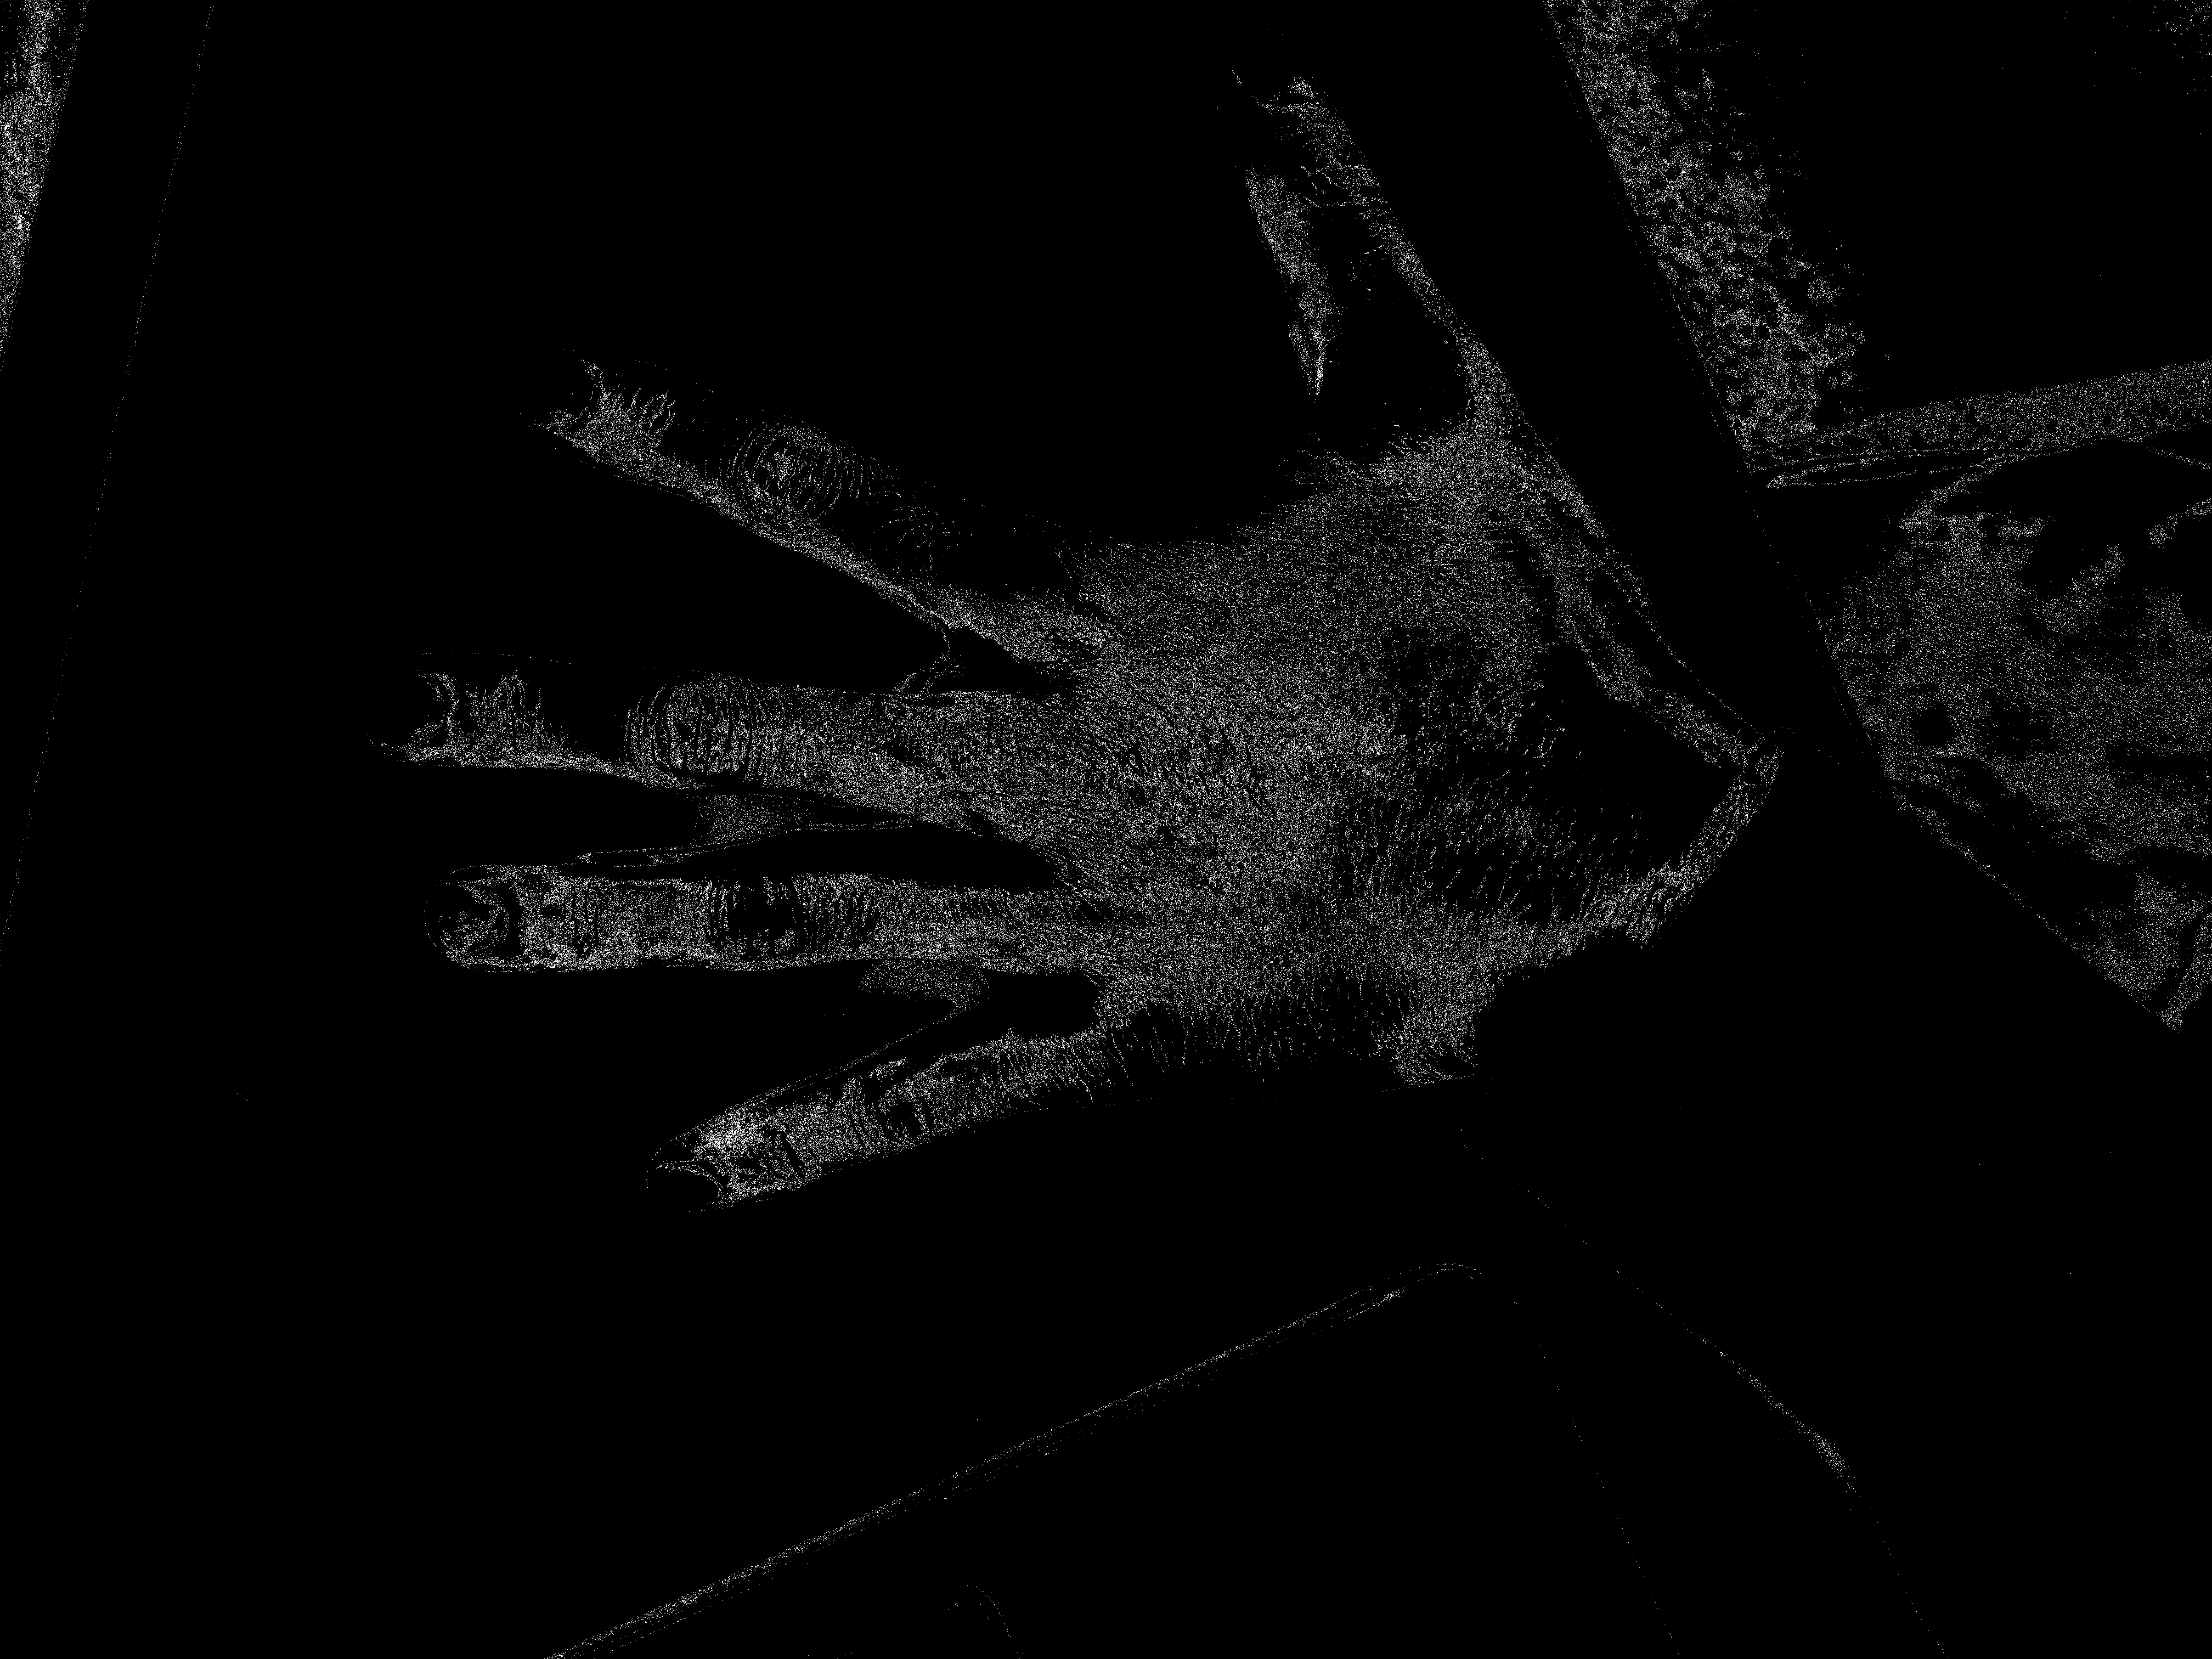
\includegraphics[keepaspectratio,width=\textwidth]{../../Figures/06_53_hand.png}
        \subcaption{肌色領域の抽出(RGB)}
    \end{minipage}
    \caption{\kadaibe\ 実験結果}
\end{figure}
\begin{figure}[H]
    \centering
    \renewcommand{\arraystretch}{1.5}
    \begin{tabularx}{\textwidth}{p{.05\textwidth}CCC}
                                                                                                & {\small 縞数\(4\)} & {\small 縞数\(16\)} & {\small 縞数\(64\)} \\
        \begin{minipage}{.05\textwidth}
            \centering
            \rotatebox{90}{縦縞}
        \end{minipage}                                                         &
        \begin{minipage}{.25\textwidth}
            \centering
            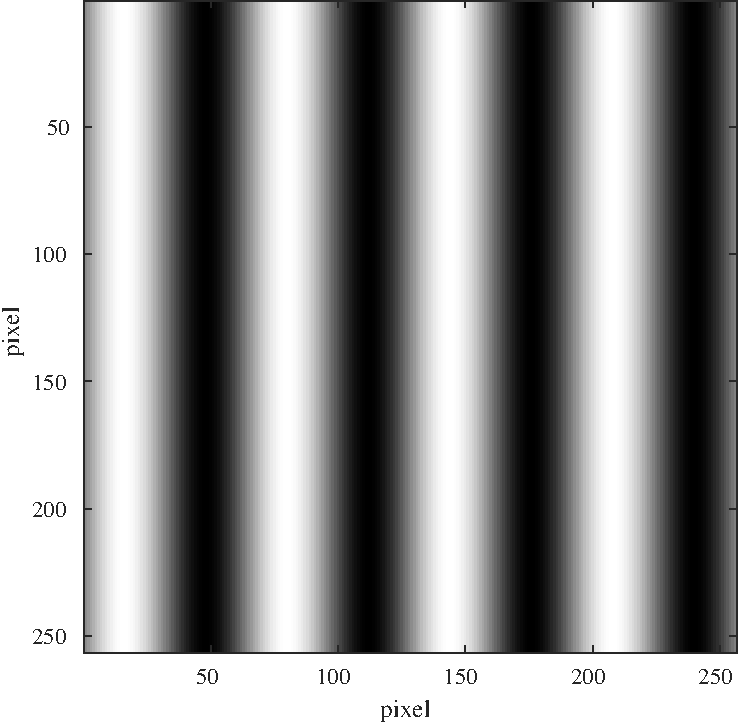
\includegraphics[width=.9\textwidth,keepaspectratio]{../../Figures/08_11_img4.pdf}
        \end{minipage}      &
        \begin{minipage}{.25\textwidth}
            \centering
            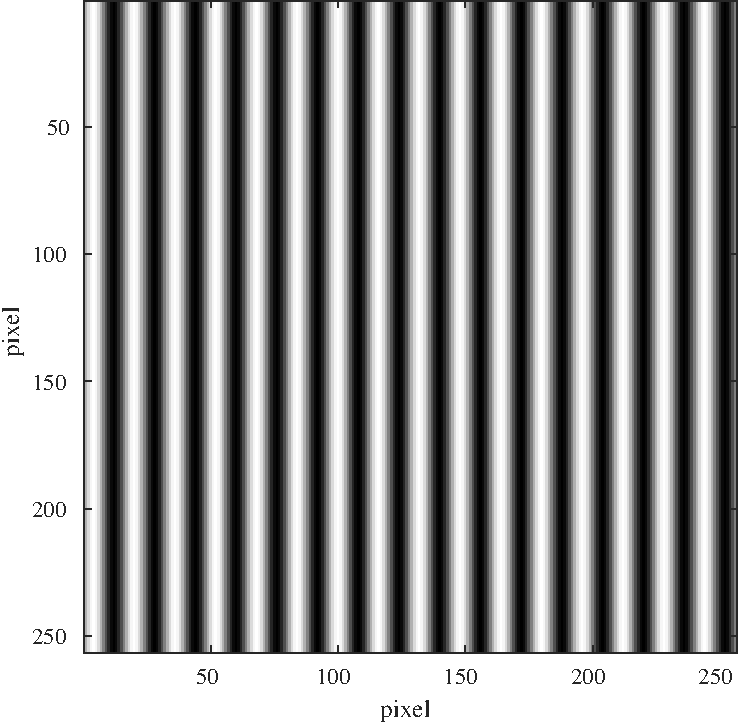
\includegraphics[width=.9\textwidth,keepaspectratio]{../../Figures/08_12_img16.pdf}
        \end{minipage}     &
        \begin{minipage}{.25\textwidth}
            \centering
            
\includegraphics[width=.9\textwidth,keepaspectratio]{../../Figures/08_13_img64.pdf}
        \end{minipage}                                                                 \\

        \begin{minipage}{.05\textwidth}
            \centering
            \rotatebox{90}{\small 縦縞\ パワースペクトル}
        \end{minipage}                                                     &
        \begin{minipage}{.25\textwidth}
            \centering
            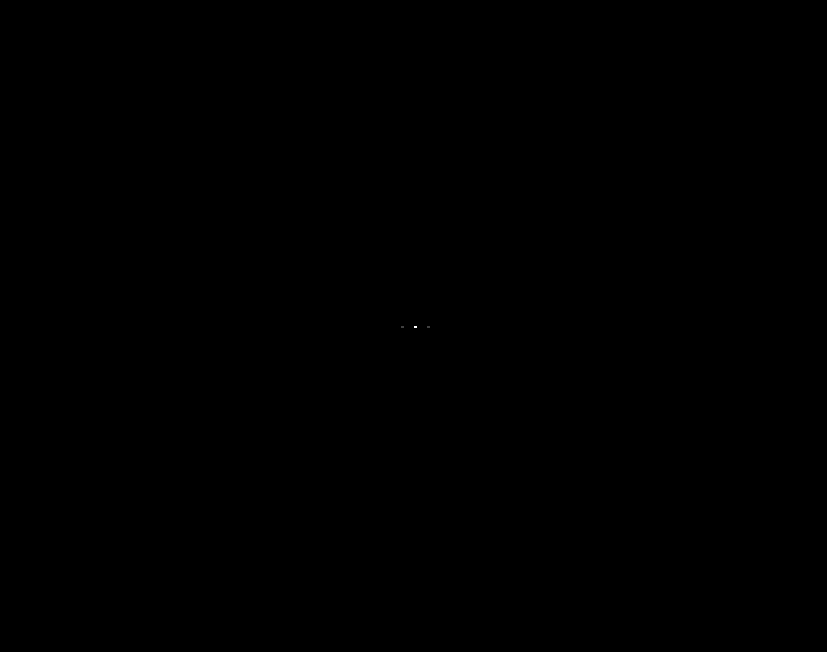
\includegraphics[keepaspectratio,width=.9\textwidth]{../../Figures/08_14_img4-fft.pdf}
        \end{minipage}  &
        \begin{minipage}{.25\textwidth}
            \centering
            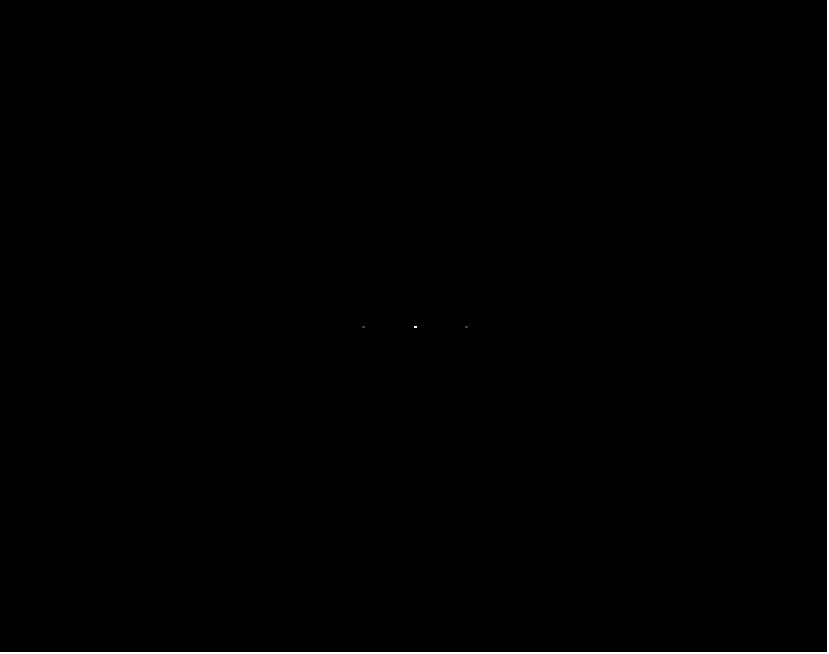
\includegraphics[keepaspectratio,width=.9\textwidth]{../../Figures/08_15_img16-fft.pdf}
        \end{minipage} &
        \begin{minipage}{.25\textwidth}
            \centering
            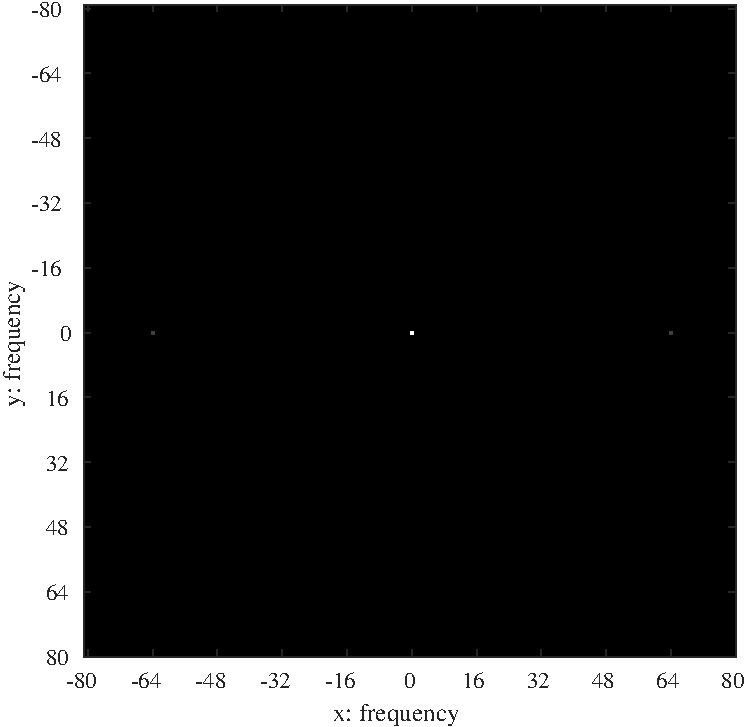
\includegraphics[keepaspectratio,width=.9\textwidth]{../../Figures/08_16_img64-fft.pdf}
        \end{minipage}                                                             \\

        \begin{minipage}{.05\textwidth}
            \centering
            \rotatebox{90}{横縞}
        \end{minipage}                                                         &
        \begin{minipage}{.25\textwidth}
            \centering
            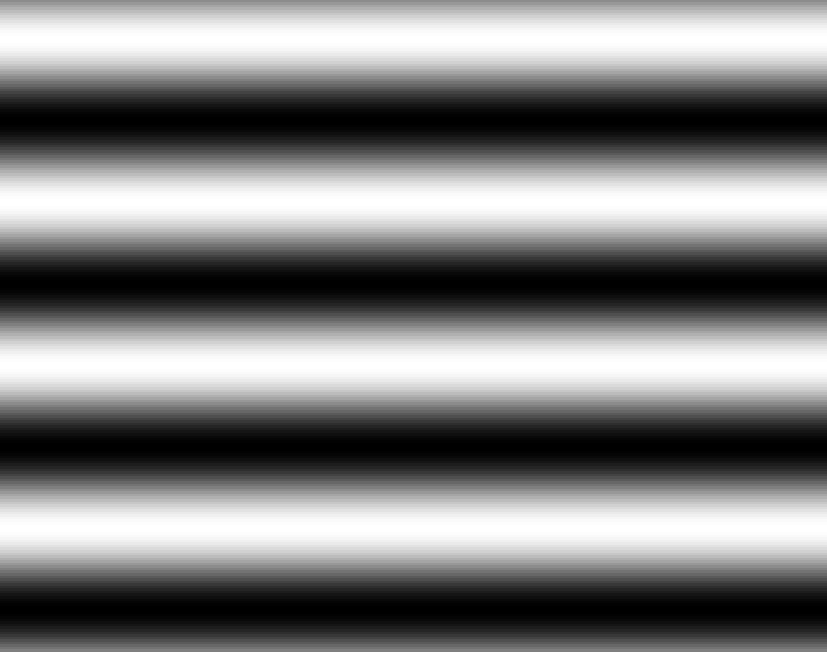
\includegraphics[width=.9\textwidth,keepaspectratio]{../../Figures/08_21_img4.pdf}
        \end{minipage}      &
        \begin{minipage}{.25\textwidth}
            \centering
            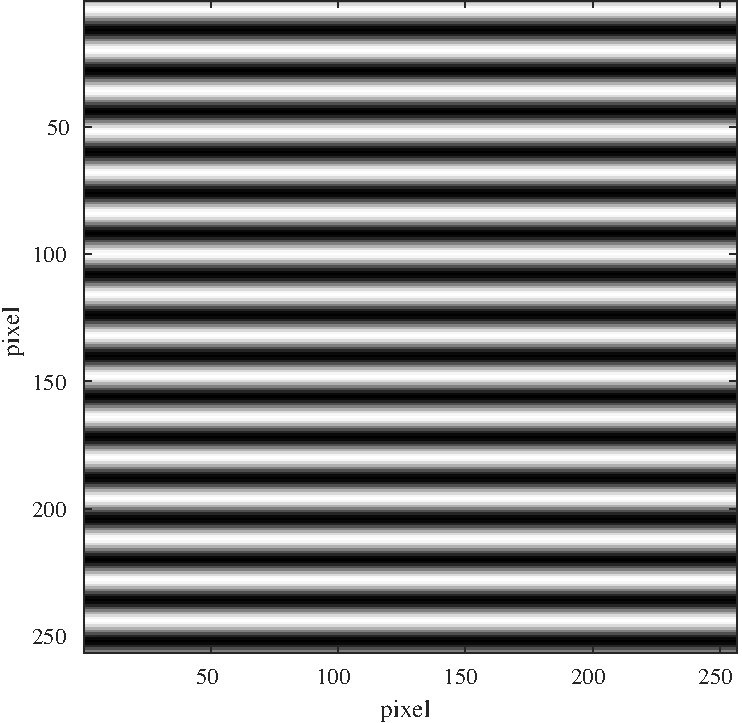
\includegraphics[width=.9\textwidth,keepaspectratio]{../../Figures/08_22_img16.pdf}
        \end{minipage}     &
        \begin{minipage}{.25\textwidth}
            \centering
            
\includegraphics[width=.9\textwidth,keepaspectratio]{../../Figures/08_23_img64.pdf}
        \end{minipage}                                                                 \\

        \begin{minipage}{.05\textwidth}
            \centering
            \rotatebox{90}{\small 横縞\ パワースペクトル}
        \end{minipage}                                                     &
        \begin{minipage}{.25\textwidth}
            \centering
            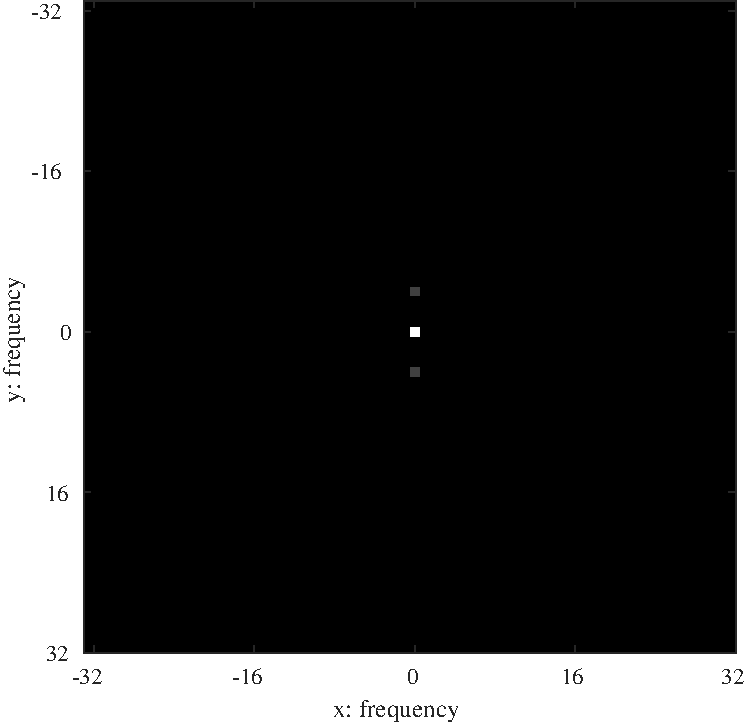
\includegraphics[keepaspectratio,width=.9\textwidth]{../../Figures/08_24_img4-fft.pdf}
        \end{minipage}  &
        \begin{minipage}{.25\textwidth}
            \centering
            \includegraphics[keepaspectratio,width=.9\textwidth]{../../Figures/08_25_img16-fft.pdf}
        \end{minipage} &
        \begin{minipage}{.25\textwidth}
            \centering
            \includegraphics[keepaspectratio,width=.9\textwidth]{../../Figures/08_26_img64-fft.pdf}
        \end{minipage}                                                             \\
    \end{tabularx}
    \caption{縦縞・横縞に対するフーリエ変換}
\end{figure}
\paragraph{2次元フーリエ変換}
両矩形の変化は,目視で確認できなかった.ただし,両パワースペクトルの差分を取った行列の最大値,最小値を調べると,いずれも\(0\)ではなかった.
\begin{figure}[H]
    \centering
    \begin{minipage}[b]{.2\textwidth}
        \centering
        \includegraphics[keepaspectratio,width=\textwidth]{../../Figures/08_31_rec1.pdf}
        \subcaption{長方形\ 1}
    \end{minipage}
    \begin{minipage}[b]{.2\textwidth}
        \centering
        \includegraphics[keepaspectratio,width=\textwidth]{../../Figures/08_32_rec2.pdf}
        \subcaption{長方形\ 2}
    \end{minipage}
    \begin{minipage}[b]{.25\textwidth}
        \centering
        \includegraphics[keepaspectratio,width=.8\textwidth]{../../Figures/08_33_rec1-fft.pdf}
        \subcaption{長方形\ 1\ パワースペクトル}
    \end{minipage}
    \begin{minipage}[b]{.25\textwidth}
        \centering
        \includegraphics[keepaspectratio,width=.8\textwidth]{../../Figures/08_34_rec2-fft.pdf}
        \subcaption{長方形\ 2\ パワースペクトル}
    \end{minipage}
    \caption{画像の座標とパワースペクトルの関係}
\end{figure}
\begin{figure}[H]
    \centering
    \begin{minipage}[b]{.23\textwidth}
        \centering
        \includegraphics[keepaspectratio,width=\textwidth]{../../LENNA.jpeg}
        \subcaption{元画像}
    \end{minipage}
    \begin{minipage}[b]{.23\textwidth}
        \centering
        \includegraphics[keepaspectratio,width=\textwidth]{../../Figures/08_41_filter.pdf}
        \subcaption{円形フィルタ\footnotemark[1]}
    \end{minipage}
    \begin{minipage}[b]{.23\textwidth}
        \centering
        \includegraphics[keepaspectratio,width=\textwidth]{../../Figures/08_42_fft.pdf}
        \subcaption{\scriptsize パワースペクトル}
    \end{minipage}
    \begin{minipage}[b]{.23\textwidth}
        \centering
        \includegraphics[keepaspectratio,width=\textwidth]{../../Figures/08_43_fft-filter.pdf}
        \subcaption{フィルタの適用\footnotemark[1]}
    \end{minipage}
    \begin{minipage}[b]{.48\textwidth}
        \centering
        \includegraphics[keepaspectratio,width=\textwidth]{../../Figures/08_44_fft-filter-50.pdf}
        \subcaption{\scriptsize フィルタ適用後\((50)\)}
    \end{minipage}
    \begin{minipage}[b]{.48\textwidth}
        \centering
        \includegraphics[keepaspectratio,width=\textwidth]{../../Figures/08_45_fft-filter-100.pdf}
        \subcaption{\scriptsize フィルタ適用後\((100)\)}
    \end{minipage}
    \caption{高域通過フィルタ}
\end{figure}
\footnotetext[1]{例として,半径が\(50\textrm{pixel}\)のフィルタを示す.}
\section{\consideration}
講義一覧,折れ線グラフ,円グラフのコンテンツを,すべての色覚で内容を判別できるように配色した.
折れ線グラフについては,マークの形状を商品別に変更することで,商品を区別した.
マークは線と同化し,一部見にくいので,線の形状やマークの色を変更することで,さらに見やすいデザインになる.
また,円グラフは,色の変更だけでなく,項目間の感覚を開けることで,色の境界に対して見やすさを保証できる.
\paragraph{色覚}
一般色覚(C型色覚)の人は,L(赤)錐体,M(緑)錐体,S(青)錐体の3種類を持っており,すべて正常に働いている.
色弱者(色の配慮が不十分な社会における弱者)は,いずれかの錐体がない,またはいずれかの錐体が不十分な働きである.
たとえば,M錐体がない,または不十分な働きであるD型色覚では,\figref{fig:D型色覚の周波数に対する感度}のように2つの周波数領域で混同が生じる.
\begin{figure}[H]
    \centering
    \begin{tikzpicture}
        \draw[thick,-latex](-.3,0)--(6.5,0)node[midway,below=.4cm]{\small 光の波長(nm)};
        \draw[thick,-latex](-.3,0)--(-.3,3)node[midway,left]{\small \rotatebox{90}{光に対する感度}};
        \foreach \u \v in {0/400,1/450,2/500,3/550,4/600,5/650,6/700}
        \draw(\u,-0.1)node[below]{\scriptsize \v}--(\u,0);
        \foreach \u in {0,0.2,...,6}
        \draw(\u,0)--(\u,0.1);
        \foreach \u in {0.3,0.6,...,3.0}
        \draw(-.3,\u)--(-.2,\u);
        \draw[very thick,blue,dotted]plot[smooth,tension=0.7]coordinates{(0,1.8)(0.8,2.7)(2.8,0.6)(4.8,0)};
        \draw[very thick,gray!80,dashed]plot[smooth,tension=0.7]coordinates{(0,0.6)(0.4,1.2)(0.8,1.5)(2.8,2.7)(5.6,0.3)};
        \draw[very thick,red,densely dash dot dot]plot[smooth,tension=0.7]coordinates{(0,0.6)(0.4,1.2)(1,1.45)(3.2,2.8)(6,0.6)};
        \draw(0.4,0)--(0.4,3);
        \draw(0.8,0)--(0.8,3);
        \draw[latex-latex](0.4,0.6)--(0.8,0.6)node[above right]{\tiny 混同};
        \draw(3.8,0)--(3.8,3);
        \draw(2.8,0)--(2.8,3);
        \draw[latex-latex](2.8,0.6)--(3.8,0.6)node[midway,above]{\tiny 混同};
    \end{tikzpicture}
    \begin{tikzpicture}
        \draw[very thick,blue,dotted](0,0)--(2,0)node[right,color=black]{青に敏感な視細胞(S錐体)};
        \draw[very thick,gray!80,dashed](0,-.5)--(2,-.5)node[right,color=black]{機能しない緑に敏感な視細胞(M錐体)};
        \draw[very thick,red,densely dash dot dot](0,-1)--(2,-1)node[right,color=black]{赤に敏感な視細胞(L錐体)};
    \end{tikzpicture}
    \caption{D型色覚の周波数に対する感度(概略)\cite{色覚が変化するとどのように色が見えるのか2}}
    \label{fig:D型色覚の周波数に対する感度}
\end{figure}
C型色覚の場合は,L錐体,M錐体,S錐体それぞれからの入力に対して比を取り,色を弁別している.
それに対して,D型色覚の場合は,L錐体とS錐体の入力の比で色を弁別しているため,L錐体とS錐体の比が同じ箇所は,色の区別がつかないと考えられる.
この混同部分を避けるために,L錐体とS錐体の感度比が異なる部分を採用する必要があるだろう.
\\\hfill\cite{色覚が変化するとどのように色が見えるのか}
\chapter{\kadaic}
\section{\purpose}
運動残効は以下のように説明されている.
\begin{quote}
    ``ある一定方向への運動をしばらく注視した後に,静止した物体を観測すると,それが逆方向に動いて見える現象.''\\
    \hfill\cite[p.58]{認知心理学辞典}
\end{quote}
方位残効とは,ある方向に傾いた線分を眺めて順応した後,テスト垂直の線分を見ると,順応刺激と反対の方向に傾いて知覚される現象である\cite[p.5]{方位残効と運動残効のメカニズム}.
また,方位選択性とは,大脳皮質視覚野細胞は受容野に特定の傾き(方位)線分刺激を提示したときに応答し,それと異なる傾きの刺激には応答しないことをいう\cite[p.764]{認知心理学辞典}.\par
今回の実験では,方位の大きさと,残効の度合いを比較し,視覚情報処理を考慮したうえで,現象について考察する.
\section{\method}
\paragraph{\kadaica}
方位を定義できる正弦波縞を作成する.
方位\(\theta\),空間周波数\(f\),コントラスト\(C\)の正弦波縞は\eqref{equ:正弦波縞}で表せる.
\(L(x,y)\)を点\(L(x,y)\)における輝度,\(L_0\)を全体画像の平均輝度とする.
\begin{align}
    L(x,y) & = L_0\Bigg(1+C\sin\Big(2\pi f\big(y\sin(\theta)+x\cos(\theta)\big)\Big)\Bigg)\label{equ:正弦波縞}
\end{align}
\(y\)軸方向を基準とし,
左に\(30^\circ\)傾いた空間周波数\(0.05\textrm{cycle}/\textrm{pixel}\)の正弦波縞と,
右に\(60^{\circ}\)傾いた空間周波数\(0.03\textrm{cycle}/\textrm{pixel}\)の正弦波を作成する.
平均輝度は,最大輝度の\(0.5\)倍,コントラストを\(0.5\)とする.
\paragraph{\kadaicb}
方位\(90\pm 10^\circ\),\(90\pm 45^\circ\)正弦波縞の順応刺激を上下に提示して,\(60\)秒後に垂直縞\(90^\circ\)のテスト刺激を表示する.
全体画像サイズを\(\textrm{縦}900\times\textrm{横}400\textrm{pixel}\),格子縞のサイズを\(400\times 400\textrm{pixel}\),順応時に提示する中央の矩形を\(20\times 100\textrm{pixel}\),順応後の注視点を\(20\textrm{pixel}\)とする.
正弦波縞の空間周波数を\(0.03\textrm{cycle}/\textrm{pixel}\),コントラストは\(0.5\)とする.
刺激を観察する際,網膜上の,局所的な明るさの順応を避けるために,\(60\)秒の順応時間では,矩形を満遍なく見るようにする.
\begin{center}
    \begin{minipage}[t]{.48\textwidth}
        \begin{lstlisting}[caption={矩形と円の作成},label={src:矩形と円の作成}]
[w, h] = meshgrid(-199:200, 50:-1:-49);
Y2 = 255*0.95;
cir = (w.^2 + h.^2 >= 10.^2)*Y2; % 円
rct = ones(100,400); % 矩形
rct = rct * Y2;
rct(50-9:50+10,200-49:200+50)=0;
        \end{lstlisting}
    \end{minipage}
    \hspace{.5em}
    \begin{minipage}[t]{.48\textwidth}
        \begin{lstlisting}[caption={順応刺激画像の作成},label={src:順応刺激画像の作成}]
% L: 正弦波縞 90°
% L_p10,L_n10: 正弦波縞 ±10° 
% L_n45,L_p45: 正弦波縞 ±45°
dg_90 = [L; cir; L];
dg_10 = [L_p10; rct; L_n10];
dg_45 = [L_n45; rct; L_p45];
        \end{lstlisting}
    \end{minipage}
    \vspace{-.5em}
\end{center}
\newpage
\begin{wrapfigure}{r}[-1mm]{.48\textwidth}
    \vspace{-1cm}
    \begin{lstlisting}[caption={刺激画像の表示方法},label={src:刺激画像の表示方法}]
fig = figure;
set(fig, 'position',get(0,'ScreenSize'));
colormap(gray(256));
image(dg_10);
axis off;
axis image;    
    \end{lstlisting}
    \vspace{-.5cm}
\end{wrapfigure}
\paragraph{刺激画像の表示}
順応刺激画像を方位残効が生じやすいように,全画面表示にし,\(60\)秒後にテスト刺激を提示するためには,\matlab の\texttt{set}関数を用いる.
また,\(60\)秒の待機時間を\texttt{pause(60)}で設定する.\texttt{axis}を設定して,画像に軸や数値ラベルを非表示にする.
\section{\result}
\begin{figure}[h]
    \centering
    \begin{minipage}[b]{.19\textwidth}
        \centering
        \includegraphics[keepaspectratio,width=\textwidth]{../../Figures/07_10_l30.pdf}
        \subcaption{左に\(30^\circ\)}
    \end{minipage}
    \begin{minipage}[b]{.19\textwidth}
        \centering
        \includegraphics[keepaspectratio,width=\textwidth]{../../Figures/07_11_r60.pdf}
        \subcaption{右に\(60^\circ\)}
    \end{minipage}
    \begin{minipage}[b]{.19\textwidth}
        \centering
        \includegraphics[keepaspectratio,width=.8\textwidth]{../../Figures/07_21_dg90.pdf}
        \subcaption{テスト刺激}
    \end{minipage}
    \begin{minipage}[b]{.19\textwidth}
        \centering
        \includegraphics[keepaspectratio,width=.8\textwidth]{../../Figures/07_22_dg45.pdf}
        \subcaption{順応刺激\ \(90\pm 45^\circ\)}
    \end{minipage}
    \begin{minipage}[b]{.19\textwidth}
        \centering
        \includegraphics[keepaspectratio,width=.8\textwidth]{../../Figures/07_23_dg10.pdf}
        \subcaption{順応刺激\ \(90\pm 10^\circ\)}
    \end{minipage}
    \caption{生成した画像}
\end{figure}
\paragraph{方位残効}
順応刺激\(90\pm10^\circ\)は,方位残効を知覚できた.順応刺激\(90\pm45^\circ\)は,方位残効を知覚できなかった.
\section{\consideration}
運動残効は,運動方位に選択的な細胞発火の頻度が高くなることで生じる.運動残効は運動を主に処理するMT野(V5)で生じる.
方位残効のメカニズムも運動残効と同じメカニズムであるが,運動残効がMT野で生じるのに対して,方位残効は1次視覚野(V1)で生じる.
垂直方向に反応する受容野に対して,順応刺激\(90-10^\circ\)の応答と感度を,\figref{fig:方位残効のメカニズム}に示す.
垂直方向に反応する受容野について,\(90\pm n^\circ\)順応刺激の\(n\)が大きい場合,感度が抑制されても応答への影響は少ない.
\(n\)が小さい場合,その感度が抑制されると,応答が小さくなるため,方位残効を知覚しやすいと考えられる.
\begin{figure}[H]
    \centering
    \input{fig_chap21}
    \caption{方位残効のメカニズム(垂直方向に反応する受容野)}
    \label{fig:方位残効のメカニズム}
\end{figure}
\begin{tikzpicture}[remember picture,overlay]
    \draw[ultra thick,-latex](A)--(2A);
    \draw[ultra thick,-latex](B)--(2B);
\end{tikzpicture}
\chapter{関連語句}
\section{ガボールフィルタ}
ガボールフィルタとは,画像を周波数領域でテクスチャ解析する方法のひとつ.
テクスチャ解析とは,粗い,滑らか,でこぼこなどの直感的な材質を,画素強度の空間的な変動の関数として定量化する試みのことである\cite{テクスチャ解析}.
テクスチャ解析する方法として,フーリエ変換がある.フーリエ変換では画像をいくつかのブロックに区切る必要があり,対象の境界も同時に検出するという問題に対して,結果が粗くなる.
周波数の不正確さと,位置の不正確さとの積には下限があり,それを最小にするのは「ガボール関数」である.\par
ガボール関数は,サルの一次視覚野にある単純細胞の受容野特性によく似ており,ガボール関数の正弦波や余弦波の傾きを変化させることで.この受容野特性をよく再現できる.
\begin{flushright}
    \cite[p.144]{認知心理学辞典}
\end{flushright}
\section{固有顔法}
固有顔(eigenface)とは,顔画像の認識において最も有名な手法のひとつ.
顔認識では,顔を構成する部品(目や鼻,口など)の形状や,配置から特徴点を抽出して認識に利用する.しかし,照明方向や,撮影距離,表情,顔の傾きなどで顔の見え方が変わる.これらを許容したうえで正しく顔認識するには,顔画像をパターンとして扱い,統計的パターン認識手法を適用する方法がある.
まず挙げられるのが,パターン間のマッチングを用いた方法である.この方法は最も簡単なパターン認識手法であるが,画像そのものをパターンとして扱った場合,パターンの次元が大きくなる.
この問題を解決する方法として提案されたのが,固有顔である.固有顔は主成分分析によりパターンを情報圧縮し,顔画像の識別に利用している.
数枚の画像に対して,各画像から平均ベクトルを引いた集合に対して,固有値を求める.この時の固有ベクトルを固有顔と呼ぶ.\par
\hfill\cite{顔画像からの個人識別}
\section{オプティカルフロー}
視覚におけるオプティカルフローとは,前方へ移動するときの,後ろへ流れる背景のことである.
このオプティカルフローには2種類の特性があり,身体が対象へ直線的な移動時に起きる「放射状オプティカルフロー」,身体が回るときに起きる「回転性のオプティカルフロー」が存在する\cite[p.679]{人間の運動学}.\par
また,動画像処理におけるオプティカルフローとは,動画像中の物体の動きを検出して,速度をべクトルで表示する手法を指す.
フロー推定方法としてブロックマッチング法を取り上げる.ブロックマッチング法は,画像のある大きさのブロックで分割し,次フレームにおける注目ブロックとの類似度が最も大きいブロックを検出する手法である\cite{オプティカルフローを用いた画像中の野鳥検出}.
\newpage
\section{ストラクチャフロムモーション(SfM: Structure from Motion)}
\begin{wrapfigure}{r}[0mm]{.5\textwidth}
    \centering
    \vspace{-.5cm}
    \input{fig_epipora1}
    \caption{エピポーラ幾何}
    \label{fig:エピポーラ幾何}
\end{wrapfigure}
ストラクチャフロムモーション(SfM)とは,一連の2次元イメージから,3次元シーンの構造を推定するプロセスを指す.
具体的には,ドローンによる空撮写真(2次元)から3次元のデータを得るときに用いられる.
ここでは,例として2つのビュー(カメラ)によるSfMを取り上げる.
カメラ1で読み取った画像と,カメラ2で読み取った画像の対応関係を抽出した後,カメラ1に対するカメラ2の姿勢を求める.
このときに,基礎行列を計算し,エピポーラ幾何を記述する(\figref{fig:エピポーラ幾何}).
生成したエピポーラ線に対して,基礎行列を計算し,カメラ1座標におけるのカメラ2座標を出力する.
最後に,マッチする点の,3次元での位置を決定し,3次元画像として描画する.
\begin{flushright}
    \cite{SfM}
\end{flushright}
\bibliography{bib}
\chapter*{付録}
\pagestyle{appendixstyle}
\addcontentsline{toc}{chapter}{付録}
\setcounter{section}{0}
\renewcommand{\thelstlisting}{\thesection-\arabic{lstlisting}}
\renewcommand{\thesection}{\Alph{section}}
\newcommand{\secref}[1]{[#1]{#1}}
\makeatletter
\@addtoreset{lstlisting}{section}
\makeatother
\lstset{
    frame={single},
    numbers={left}
}
\section{\kadaia\ (April 27th, 2023)}
\lstinputlisting[caption={\secref{\kadaiaa}},label={src:05_01}]{../../05_UnderstandingImages/no1.m}
\lstinputlisting[caption={\secref{\kadaiab}},label={src:05_02}]{../../05_UnderstandingImages/no2.m}
\lstinputlisting[caption={\secref{\kadaiac}},label={src:05_03}]{../../05_UnderstandingImages/no3.m}
\lstinputlisting[caption={\secref{\kadaiad}},label={src:05_04}]{../../05_UnderstandingImages/no4.m}
\lstinputlisting[caption={\secref{\kadaiae}},label={src:05_05}]{../../05_UnderstandingImages/no5.m}
\lstinputlisting[caption={\secref{\kadaiaf}},label={src:05_06}]{../../05_UnderstandingImages/no6.m}
\section{\kadaib\ (May 8th, 2023)}
\lstinputlisting[caption={\secref{\kadaiba}},label={src:06_01}]{../../06_ImageFiltering/no1.m}
\lstinputlisting[caption={\secref{\kadaibb}},label={src:06_02}]{../../06_ImageFiltering/no2.m}
\lstinputlisting[caption={\secref{\kadaibc}},label={src:06_03}]{../../06_ImageFiltering/no3.m}
\lstinputlisting[caption={\secref{\kadaibd}},label={src:06_04}]{../../06_ImageFiltering/no4.m}
\lstinputlisting[caption={\secref{\kadaibe}},label={src:06_05}]{../../06_ImageFiltering/no5.m}
\lstinputlisting[caption={\secref{\kadaibd}\ \texttt{fucntion}},label={src:06_05_f}]{../../06_ImageFiltering/no5_hsvfunc.m}
\section{\ (April 20th, 2023)}
\section{\ (April 24th, 2023)}
\end{document}